\documentclass[11pt]{article}
\usepackage[T1]{fontenc}
\usepackage[utf8]{inputenc}
\usepackage{lmodern}
\usepackage[margin=1in]{geometry}
\usepackage{amsmath,amssymb,amsthm,mathtools}
\def\DoNotLoadEpstopdf{}
\usepackage{graphicx}
\usepackage{tikz}
\usetikzlibrary{arrows.meta,positioning,calc}
\usepackage{microtype}
\usepackage{xurl}
\usepackage[colorlinks=true,linkcolor=blue!45!black,citecolor=blue!45!black,urlcolor=blue!45!black]{hyperref}
\usepackage{bookmark}
\hypersetup{
  pdftitle={The Euclidean Steinitz--Bergstr\"om theorem},
  pdfauthor={OpenAI}
}
\newtheorem{theorem}{Theorem}[section]
\newtheorem{proposition}[theorem]{Proposition}
\newtheorem{lemma}[theorem]{Lemma}
\newtheorem{corollary}[theorem]{Corollary}
\theoremstyle{definition}
\newtheorem{definition}[theorem]{Definition}
\theoremstyle{remark}
\newtheorem{remark}[theorem]{Remark}
\newcommand{\R}{\mathbb R}
\newcommand{\Z}{\mathbb Z}
\newcommand{\HS}{\mathrm{HS}}
\newcommand{\op}{\mathrm{op}}
\DeclareMathOperator{\tr}{tr}
\DeclareMathOperator{\supp}{supp}
\DeclareMathOperator{\diag}{diag}
\title{The Euclidean Steinitz--Bergstr\"om theorem}
\author{OpenAI}
\date{September 24, 2026}
\begin{document}
\maketitle
\begin{abstract}
Every prescribed-order finite sequence of vectors in the Euclidean unit
ball of $\R^d$ has one signing for which every signed prefix has norm at
most $C\sqrt d$, with $C$ absolute and independent of the sequence length.
Consequently, every indexed zero-sum family of unit-ball vectors admits an
ordering with the same bound for its unsigned partial sums. This determines
the Euclidean Steinitz constant up to absolute factors,
$S_2(d)=\Theta(\sqrt d)$, and resolves the Euclidean
Steinitz--Bergstr\"om conjecture.
\end{abstract}
{\small\tableofcontents}
\clearpage
\section{Introduction}

Let $v_1,\ldots,v_N$ be vectors in the Euclidean unit ball of $\R^d$.
There are two natural ways to keep their partial sums small: choose signs
in a prescribed order, or, when the family sums to zero, choose an order
without changing any signs. The difficulty in the first problem is to
control every prefix by one choice of signs, with a bound independent of
$N$. We prove such a bound on the square-root scale in the dimension.

\begin{theorem}[Prescribed-order signed prefixes]\label{thm:signing}
There is an absolute constant $C$ such that, for all integers $d,N\ge1$ and
every sequence $v_1,\ldots,v_N\in\R^d$ with $\lVert v_i\rVert_2\le1$,
there are signs $\varepsilon_1,\ldots,\varepsilon_N\in\{-1,1\}$ for which
\[
 \max_{0\le k\le N}
 \left\lVert\sum_{i=1}^k\varepsilon_i v_i\right\rVert_2\le C\sqrt d.
\]
The same signs control all prefixes, and $C$ is independent of $d$, $N$
and the sequence.
\end{theorem}

The zero-sum ordering problem is quantified by the Euclidean Steinitz
constant. For an indexed family with $\sum_{i=1}^N v_i=0$, define
\[
 \beta(v_1,\ldots,v_N)
 =\min_{\pi\in\mathfrak S_N}\;
   \max_{0\le k\le N}\left\lVert\sum_{i=1}^k v_{\pi(i)}\right\rVert_2,
\]
where $\mathfrak S_N$ is the set of permutations of $\{1,\ldots,N\}$
and an empty sum is zero. Let $S_2(d)$ be the supremum of $\beta$ over
all finite indexed zero-sum families of Euclidean unit-ball vectors in
$\R^d$. The Euclidean Steinitz--Bergstr\"om conjecture asks whether
$S_2(d)=O(\sqrt d)$. Theorem~\ref{thm:signing} gives its affirmative resolution.

\begin{theorem}[Euclidean Steinitz--Bergstr\"om bound]\label{thm:steinitz}
There is an absolute constant $C$ such that, for all integers $d,N\ge1$ and
every indexed family $v_1,\ldots,v_N\in\R^d$ satisfying
$\lVert v_i\rVert_2\le1$ and $\sum_{i=1}^N v_i=0$, some permutation
$\pi\in\mathfrak S_N$ satisfies
\[
 \max_{0\le k\le N}\left\lVert\sum_{i=1}^k v_{\pi(i)}\right\rVert_2
 \le C\sqrt d.
\]
The constant in Theorem~\ref{thm:signing} also suffices here.
\end{theorem}

Both statements allow repetitions and zero vectors. The empty-sequence
and dimension-zero extensions have every partial sum equal to zero. The construction is
existential: its choices may depend on the complete input sequence. Its
successive choice of signs does not supply an online rule or an efficient
algorithm.

The order of growth in Theorem~\ref{thm:steinitz} is necessary. In the
$d$-dimensional hyperplane orthogonal to the all-ones vector
$\mathbf1\in\R^{d+1}$, let $e_i$ denote the standard coordinate vectors and take
\[
 u_i=\sqrt{\frac{d+1}{d}}\left(e_i-\frac{\mathbf1}{d+1}\right),
 \qquad 1\le i\le d+1.
\]
These unit vectors sum to zero and satisfy $\langle u_i,u_j\rangle=-1/d$
for $i\ne j$. Hence every sum of $k$ distinct members has squared norm
$k(d+1-k)/d$. With $k=\lfloor(d+1)/2\rfloor$, this is at least $d/4$,
regardless of the ordering. Thus
\[
 \tfrac12\sqrt d\le S_2(d)\le C\sqrt d\qquad(d\ge1).
\]

\subsection{From signs to an ordering}

We give the short transference argument at once. Chobanyan's
transference principle~\cite{Chobanyan1994} relates rearrangements and
signed sums. We use its finite positive-forward, negative-reverse form
\cite[Theorem~2.1 and Remark~1]{ChobanyanEtAl2023}.

\begin{proof}[Proof of Theorem~\ref{thm:steinitz} from Theorem~\ref{thm:signing}]
Fix an indexed zero-sum family and choose an order attaining its minimum
$\beta$; this exists because there are only finitely many permutations.
Relabel the vectors in that order. Put
\[
 A_j=\sum_{i=1}^jv_i,
 \qquad B_j=\sum_{i=1}^j\varepsilon_i v_i,
 \qquad 0\le j\le N,
\]
where the signs come from Theorem~\ref{thm:signing}. Hence
$\lVert A_j\rVert_2\le\beta$ and $\lVert B_j\rVert_2\le C\sqrt d$.
The positive-sign and negative-sign selections from an original prefix
sum respectively to
\[
 P_j=\frac{A_j+B_j}{2},\qquad M_j=\frac{A_j-B_j}{2}.
\]
Place all positive-sign indices in their original order, followed by all
negative-sign indices in reverse original order. A partial sum in the
first block is some $P_j$. In the second block, the unused indices are
the negative-sign indices of an original prefix. Since the total sum
is zero, the current partial sum is therefore some $-M_j$. This also
covers either block being empty. Every new partial sum has norm at most
$(\beta+C\sqrt d)/2$. By minimality,
\[
 \beta\le\frac{\beta+C\sqrt d}{2},
 \qquad\text{and hence}\qquad \beta\le C\sqrt d.
\]
This permutes indices and so preserves all multiplicities.
\end{proof}

The signed-prefix bound also yields finite-dimensional $\ell_p$ estimates
and a colorful row-permutation theorem. We develop these distinct
consequences in Section~\ref{sec:consequences}.

\subsection{Historical context}

The finite rearrangement theorem goes back to Steinitz's work on
conditionally convergent vector series; Ambrus and Heck give a historical
account in \cite[Section~2]{AmbrusHeck2026}.
The dimension bound for zero-sum rearrangement holds for arbitrary norms:
Grinberg and Sevast'yanov~\cite[Theorem~1]{GrinbergSevastyanov1980} prove
that the partial sums can be kept within $d$ times the unit ball.
The smaller square-root scale in Euclidean space has a long history;
Behrend discusses this expected growth in
\cite[p.~108]{Behrend1954}. The modern formulation and its attribution
to Bergstr\"om are recorded by Ambrus and Heck
\cite[Conjecture~5]{AmbrusHeck2026}. Their Theorem~7 reduces the
asymptotic question to a relaxed rearrangement problem for vectors with
norms in $[1-\varepsilon,1]$, with $0<\varepsilon\le1$ fixed independently
of the dimension. In that problem each prefix is compared with its
proportional share of the total sum, rather than with zero.
For prescribed-order Euclidean signing, the square-root-dimension
question is stated explicitly by Bansal, Jiang, Meka, Singla and
Sinha~\cite[Section~6, Conjecture~6.3]{BansalEtAl2021Full}, following
Banaszczyk~\cite{Banaszczyk2012}. Their discussion records Banaszczyk's
bound $O(\sqrt d+\sqrt{\log N})$; the length term becomes significant when
$N$ is large compared with the dimension. In a 2026 preprint, Dutta, Jha
and Jiang state an efficient prescribed-order signing bound
\[
 O\bigl(\sqrt d+d^{1/4}\log^{7/4}N\bigr),
\]
and the corresponding zero-sum ordering bound
\cite[Theorem~1.1 and Corollary~1.2]{DuttaJhaJiang2026}.
Theorem~\ref{thm:signing} gives an absolute multiple of $\sqrt d$
for every finite length.

Terminal vector balancing has a different quantifier. For columns in the
Euclidean unit ball, Li~\cite[Theorem~1.1]{Li2026} bounds the final
signed sum in infinity norm by an absolute constant and gives a
deterministic polynomial-bit algorithm on rational input. That terminal
statement implies a Euclidean bound of order $\sqrt d$ for one sum.
Applying it separately to each prefix permits the signs to change with
the prefix; Theorem~\ref{thm:signing} instead supplies one common signing.
The present all-prefix estimate is Euclidean and does not assert a
constant infinity-norm all-prefix bound.

\subsection{Proof strategy}

Gaussian convex bodies are a central setting for vector balancing, notably
in the theorem of Banaszczyk~\cite{Banaszczyk1998}. Our proof takes place
in a space of coefficients: one coordinate is
reserved for each incoming vector, together with $d$ initial state
coordinates. A sequence of linear maps sends these coefficients to
states in $\R^d$. At each step an invertible contraction acts on the old
state and the next coefficient injects a multiple of the incoming vector.
The body of coefficients for which every state is bounded will provide
the simultaneous control of all prefixes.

Two analytic ingredients make this construction possible. First, if a
bounded symmetric convex body has small Dirichlet energy for every
positive diagonal weight, it supports a single square root of a probability density
with small derivatives in every coordinate. A lifted Steiner
symmetrization preserves these bounds and permits a coordinate step
of the form $q+\varepsilon$, where $|q|\le1/4$ and
$\varepsilon\in\{-1,1\}$. This adapts the directional-density and
symmetrization method of Guo, Fang and Lu
\cite[Sections~3--4]{GuoFangLu2026}.\footnote{Guo, Fang and Lu
credit the Odin Automatic AI Research Agent for their proof.}
Bandeira~\cite{Bandeira2026} gives a related formulation for terminal
balancing in terms of Dirichlet eigenvalues. Akbas and Sra
\cite[Lemmas~2.2--2.3]{AkbasSra2026} develop the common quadratic-energy
witness and lifted $L^2$-symmetrization argument. Here the hypotheses use
diagonal weights, and the coordinate shifts may depend on earlier choices.
We prove the required energy and shifted-step statements in full.

Second, the filtered body has a diagonal Dirichlet-energy bound
independent of the number of filters. To prove this, we follow a stationary Ornstein--Uhlenbeck process
in coefficient space and localize its filtered states to dyadic spectral
scales. A matrix estimate controls changes at one scale by an additive
trace budget, including gains inserted between noncommuting contractions.
At a fixed scale, this estimate gives a uniform positive probability
for all constraints in a group of indices with bounded accumulated energy,
over a matched time interval. Gaussian correlation combines these groups,
scales and time intervals; the exponential survival rate yields the energy
bound.

The two ingredients meet through a scalar predictor. The allowed shift
in the incoming coefficient exactly compensates for the contraction of
the old state. Consequently the final states are the signed partial
sums themselves. We give this complete construction in
Section~\ref{sec:construction}, after stating the two analytic
propositions. Section~\ref{sec:shifted-signs} proves the shifted-sign proposition.
Section~\ref{sec:matrix} establishes the matrix variation estimate, and
Section~\ref{sec:survival} uses it to prove the filtered-body energy bound.
Section~\ref{sec:consequences} develops the norm-comparison and colorful
row-permutation consequences.

Throughout, all unspecified constants are absolute. Vectors and matrices
are real; $\lVert\cdot\rVert_\op$ and $\lVert\cdot\rVert_\HS$ denote
operator and Hilbert--Schmidt norms. For symmetric matrices, $A\le B$
means that $B-A$ is positive semidefinite. Functions of positive definite
matrices are defined by the spectral calculus.

\section{Constructing the signed walk}\label{sec:construction}

We will encode the signed walk by one point in a convex body in a larger
coefficient space.  The body controls a contracted version of every prefix.
Its extra coordinates will be chosen so that their contributions exactly
restore the parts removed by the contractions.  This section states the two
analytic inputs and proves Theorem~\ref{thm:signing} from them.

\subsection{The two analytic inputs}

Let $D\subset\R^m$ be a nonempty bounded open convex set, and let $Q$ be a
positive definite diagonal $m\times m$ matrix.  Define its diagonal Dirichlet
energy by
\begin{equation}\label{eq:dirichlet-energy}
 \lambda_Q(D)=
 \inf_{0\ne g\in H^1_0(D)}
 \frac{\displaystyle\int_D\langle Q\nabla g,\nabla g\rangle\,dx}
      {\displaystyle\int_Dg^2\,dx}.
\end{equation}
Here $H^1_0(D)$ is the closure of $C_c^\infty(D)$ in the Sobolev norm, and
derivatives are weak derivatives.  This normalization corresponds to
Brownian motion with covariance rate $2Q$.  Central symmetry will always
mean symmetry about the origin.  Fix
\begin{equation}\label{eq:signing-constants}
 \kappa=\frac1{100},\qquad \delta=\frac14.
\end{equation}

Our first input turns small coordinate energies into signs while allowing a
bounded shift at each step.  The shifts may depend on previously assigned
coordinates.

\begin{proposition}[Signs with adaptive shifts]\label{prop:adaptive}
Let $K\subset\R^m$ be nonempty, bounded, open, convex and centrally
symmetric.  Suppose that
\begin{equation}\label{eq:all-diagonal-energy}
 \lambda_Q(K)\le\kappa^2\tr Q
 \quad\text{for every positive definite diagonal }Q.
\end{equation}
Let $j_1,\ldots,j_s$ be distinct elements of $\{1,\ldots,m\}$, and let
$q_i:\R^{i-1}\to[-\delta,\delta]$ be arbitrary functions, for
$1\le i\le s$.  There exist signs $\varepsilon_1,\ldots,\varepsilon_s$
such that the recursion
\[
 x^{(0)}=0,\qquad
 x^{(i)}=x^{(i-1)}+
 \bigl(q_i(x^{(i-1)}_{j_1},\ldots,x^{(i-1)}_{j_{i-1}})
       +\varepsilon_i\bigr)e_{j_i}
\]
has $x^{(s)}\in K$.  For $i=1$, the function $q_1$ has a one-point domain.
\end{proposition}

This is an existence statement; the choice of signs can depend on the whole
body $K$ and all the prescribed functions.  Its proof uses backward
transformations of $K$, followed by forward choices of the signs.

The second input supplies a body satisfying a uniform energy bound.  Its
linear maps retain a $d$-dimensional state and read one new coordinate at
each step.

\begin{proposition}[Energy of a filtered path body]\label{prop:filtered}
There are positive absolute constants $A_0,B_0,H_0$ with the following
property.  Let $d\ge1$ and $n\ge0$ be integers and put $m=d+n$.  For
$1\le t\le n$, let $C_t$ be an invertible real $d\times d$ matrix and let
$b_t\in\R^d$ satisfy
\[
 C_tC_t^T+b_tb_t^T=I_d.
\]
Define linear maps $R_t:\R^m\to\R^d$ by
\begin{equation}\label{eq:filter-recursion}
 R_0x=(x_1,\ldots,x_d),\qquad
 R_tx=C_tR_{t-1}x+b_tx_{d+t}\quad(1\le t\le n).
\end{equation}
Then the bounded open convex centrally symmetric set
\begin{equation}\label{eq:filtered-body}
 \mathcal D=
 \left\{x\in\R^m:
 \begin{array}{ll}
 |x_j|<B_0 & (1\le j\le m),\\
 \lVert R_tx\rVert_2<A_0\sqrt d & (0\le t\le n)
 \end{array}\right\}
\end{equation}
satisfies
\[
 \lambda_Q(\mathcal D)\le H_0\tr Q
 \quad\text{for every positive definite diagonal }Q.
\]
\end{proposition}

The constants are independent of the number of maps and of $Q$.  This
uniformity is essential: the application will use $n$ equal to the number
of vectors.  To compensate for the contractions, we will also impose linear
constraints on the coefficients.  The following estimate bounds their
additional energy cost; we prove it after completing the construction.

\begin{lemma}[Adding slabs]\label{lem:slab-energy}
Let $D\subset\R^m$ be bounded, nonempty, open, convex and centrally
symmetric.  Let $D_*>0$, $\delta>0$, and let $m_1,\ldots,m_n$ be real
rows of length $m$.  Set
\[
 K=(2D_*D)\cap\bigcap_{i=1}^n\{x:|m_i x|<\delta\}.
\]
For every positive definite diagonal $Q$,
\begin{equation}\label{eq:slab-energy}
 \lambda_Q(K)
 \le D_*^{-2}\lambda_Q(D)
     +\pi^2\delta^{-2}\sum_{i=1}^n m_iQm_i^T.
\end{equation}
\end{lemma}

\subsection{The filter, the shifts, and their cancellation}

We now prove the signed-prefix theorem from
Propositions~\ref{prop:adaptive} and~\ref{prop:filtered}.  Their proofs in the
remaining sections are independent of this application.

\begin{proof}[Proof of Theorem~\ref{thm:signing}]
Write the prescribed sequence as $v_1,\ldots,v_n\in\R^d$, with
$\lVert v_i\rVert_2\le1$.  The hypotheses give $d,n\ge1$.

\paragraph{The symmetric contractions.}
For a positive absolute $\sigma<1$, to be chosen below, set
\begin{equation}\label{eq:symmetric-filter}
 b_i=\sigma v_i,\qquad
 \eta_i=\frac1{1+\sqrt{1-\lVert b_i\rVert_2^2}},\qquad
 C_i=I-\eta_ib_ib_i^T.
\end{equation}
On the span of $b_i$, the matrix $C_i$ has eigenvalue
$\sqrt{1-\lVert b_i\rVert_2^2}$, and on its orthogonal complement it is the
identity.  This includes $b_i=0$, for which $\eta_i=1/2$ and $C_i=I$.
Consequently
\[
 C_i=(I-b_ib_i^T)^{1/2}=C_i^T\succ0,
 \qquad C_i^2+b_ib_i^T=I,
 \qquad \frac12\le\eta_i\le1.
\]
Use these matrices in~\eqref{eq:filter-recursion}, and let $\mathcal D$ be
the body in Proposition~\ref{prop:filtered}.

For $x\in\R^{d+n}$, let $x^0$ be obtained by setting its first $d$
coordinates to zero.  Define row vectors $m_i$ by
\begin{equation}\label{eq:predictor-rows}
 m_ix=\eta_i b_i^TR_{i-1}x^0.
\end{equation}
Each row $m_i$ is supported only on the noise coordinates
$d+1,\ldots,d+i-1$.  In particular it is unaffected by any coordinate
assigned at step $i$ or later.

\paragraph{The cost of the predictor constraints.}
Let $M$ be the matrix with rows $m_i$.  We claim that every column of $M$
has squared Euclidean norm at most $\sigma^2$.  Its initial $d$ columns are
zero.  For a noise coordinate $d+j$, follow its contribution to the state:
\[
 r_j=b_j,\qquad r_i=C_ir_{i-1}\quad(j<i\le n).
\]
The coefficient of that coordinate in $m_i$ is zero for $i\le j$, and is
$\eta_i b_i^Tr_{i-1}$ for $i>j$.  Symmetry of $C_i$ gives the exact loss
identity
\[
 \lVert r_{i-1}\rVert_2^2-\lVert r_i\rVert_2^2
 =(b_i^Tr_{i-1})^2.
\]
Thus the losses telescope:
\begin{equation}\label{eq:predictor-columns}
 \begin{aligned}
 \lVert Me_{d+j}\rVert_2^2
 &=\sum_{i=j+1}^n\eta_i^2(b_i^Tr_{i-1})^2\\
 &\le\sum_{i=j+1}^n
       \bigl(\lVert r_{i-1}\rVert_2^2-\lVert r_i\rVert_2^2\bigr)
 \le\lVert b_j\rVert_2^2\le\sigma^2.
 \end{aligned}
\end{equation}
In particular, for every positive definite diagonal $Q$,
\begin{equation}\label{eq:predictor-weighted-cost}
 \sum_{i=1}^n m_iQm_i^T
 =\sum_{j=1}^{d+n}Q_{jj}\lVert Me_j\rVert_2^2
 \le\sigma^2\tr Q.
\end{equation}

Choose an absolute dilation $D_*>0$ and define
\begin{equation}\label{eq:application-body}
 K=(2D_*\mathcal D)\cap
   \{x:|m_ix|<\delta\text{ for }1\le i\le n\}.
\end{equation}
This is a bounded open convex centrally symmetric set containing a
neighborhood of zero.  Lemma~\ref{lem:slab-energy},
Proposition~\ref{prop:filtered}, and~\eqref{eq:predictor-weighted-cost} give
\begin{equation}\label{eq:application-energy}
 \lambda_Q(K)
 \le\left(H_0D_*^{-2}+\pi^2\delta^{-2}\sigma^2\right)\tr Q.
\end{equation}
We can therefore fix, once and for all,
\begin{equation}\label{eq:absolute-parameters}
 D_*\ge\max\{1,\sqrt{2H_0}/\kappa\},\qquad
 \sigma=\min\{1/2,\kappa\delta/(\sqrt2\pi)\}.
\end{equation}
The same body $K$ then satisfies~\eqref{eq:all-diagonal-energy} for every
positive definite diagonal $Q$.  These choices are independent of $d$, $n$
and the vectors.

\paragraph{Choosing the coefficients.}
For $u\in\R$ write
$\operatorname{clip}_\delta(u)=\max\{-\delta,\min\{u,\delta\}\}$.
Apply Proposition~\ref{prop:adaptive} to the distinct axes
$e_{d+1},\ldots,e_{d+n}$.  At step $i$ prescribe the shift
\[
 q_i=\operatorname{clip}_\delta(m_ix^{(i-1)}).
\]
By the support of $m_i$, this is a function of the previously assigned
coordinates, as required.  The proposition supplies signs and a final point
$x=x^{(n)}\in K$.  Its first $d$ coordinates remain zero.  Also, coordinates
assigned before step $i$ never change afterward, so
\[
 m_ix^{(i-1)}=m_ix.
\]
The final membership $x\in K$ implies $|m_ix|<\delta$.  Hence each shift
was already within the permitted interval: clipping was inactive, and
\begin{equation}\label{eq:unclipped-coordinates}
 x_{d+i}=m_ix+\varepsilon_i
 =\eta_i b_i^TR_{i-1}x+\varepsilon_i.
\end{equation}
Here $x^0=x$ because the initial block is zero.  Clipping is used only to
make the application of Proposition~\ref{prop:adaptive} unconditional;
causality and the final constraints subsequently remove it.

Figure~\ref{fig:cancellation} illustrates the identity that completes the
construction.

\paragraph{Cancellation.}
For this single final coefficient vector, $R_0x=0$ and
\begin{align*}
 R_tx
 &=C_tR_{t-1}x+b_tx_{d+t}\\
 &=(I-\eta_tb_tb_t^T)R_{t-1}x
   +b_t(\eta_tb_t^TR_{t-1}x+\varepsilon_t)\\
 &=R_{t-1}x+\varepsilon_tb_t.
\end{align*}
Thus, simultaneously for every $0\le t\le n$,
\begin{equation}\label{eq:feedback-cancellation}
 R_tx=\sum_{i=1}^t\varepsilon_ib_i.
\end{equation}
Since $x\in2D_*\mathcal D$, all these states have norm less than
$2D_*A_0\sqrt d$.  Dividing~\eqref{eq:feedback-cancellation} by $\sigma$
proves Theorem~\ref{thm:signing} with the absolute constant
$C=2D_*A_0/\sigma$.
\end{proof}

\begin{figure}[htbp]
 \centering
 \resizebox{0.96\textwidth}{!}{%
 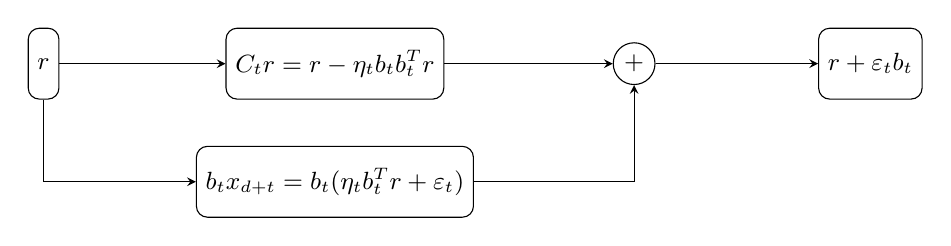
\begin{tikzpicture}[
   >=stealth,
   every node/.style={font=\small},
   state/.style={draw,rounded corners,align=center,minimum height=9mm}]
  \node[state] (r) at (0,0) {$r$};
  \node[state] (contract) at (3.7,0)
    {$C_tr=r-\eta_tb_tb_t^Tr$};
  \node[draw,circle,inner sep=2pt] (sum) at (7.5,0) {$+$};
  \node[state] (out) at (10.5,0) {$r+\varepsilon_tb_t$};
  \node[state] (incoming) at (3.7,-1.5)
    {$b_tx_{d+t}=b_t(\eta_tb_t^Tr+\varepsilon_t)$};
  \draw[->] (r) -- (contract);
  \draw[->] (contract) -- (sum);
  \draw[->] (sum) -- (out);
  \draw[->] (r.south) -- (0,-1.5) -- (incoming.west);
  \draw[->] (incoming.east) -- (7.5,-1.5) -- (sum.south);
 \end{tikzpicture}}
 \caption{For the final coefficient vector, put $r=R_{t-1}x$.
 The predictor term in the incoming coordinate restores exactly the
 component removed by $C_t$, leaving the signed increment
 $\varepsilon_tb_t$.}
 \label{fig:cancellation}
\end{figure}

\subsection{Brownian proofs of the slab bound}

We now prove Lemma~\ref{lem:slab-energy}, which bounded the cost of the
predictor constraints.  Brownian survival converts intersection with slabs
into an event to which Gaussian correlation applies.  The two Brownian
facts below will also be used in the remaining analytic arguments.

\begin{lemma}[Brownian survival rate]\label{lem:brownian-rate}
Let $D\subset\R^m$ be bounded, nonempty, open and convex, and let $Q$ be
positive definite and diagonal.  If $W$ is Brownian motion with covariance
rate $2Q$, started at $x\in D$, then
\begin{equation}\label{eq:brownian-rate}
 \lim_{T\to\infty}-\frac1T
 \log\mathbb P_x\{W(s)\in D\text{ for all }0\le s\le T\}
 =\lambda_Q(D).
\end{equation}
In particular, the starting point may be $0$ when $D$ is centrally
symmetric.
\end{lemma}

\begin{proof}
The generator of $W$ is $\tr(Q\nabla^2)$.  Let
$\tau_D=\inf\{s\ge0:W(s)\notin D\}$, and let
\[
 P_s^D h(x)=\mathbb E_x[h(W(s))\mathbf 1_{\{s<\tau_D\}}]
\]
be its killed semigroup.  The corresponding nonnegative self-adjoint
operator is the Dirichlet realization of $-\tr(Q\nabla^2)$, with form
$\int_D\nabla g^TQ\nabla g$ on $H_0^1(D)$.
These standard Dirichlet facts apply here because bounded convex domains
are connected and Lipschitz; see, for example,
\cite[Section~2 and Appendix~C]{DaviesSimon1984}, after the linear change
of coordinates for $Q$ and the time normalization above.
The killed representation can also be obtained first on smooth interior
domains and then by exhaustion: their compactly supported smooth
functions exhaust the form domain, while any continuous path remaining
in $D$ on a compact time interval has compact image in $D$.

Write $\lambda=\lambda_Q(D)$.  Compactness of
$H_0^1(D)\hookrightarrow L^2(D)$ and the spectral theorem give
$\lVert P_s^D\rVert_{2\to2}=e^{-s\lambda}$ and a first eigenfunction
$\varphi$ that can be chosen nonnegative by taking the absolute value
of a Rayleigh minimizer.  Interior elliptic regularity and the strong
maximum principle make $\varphi$ strictly positive at every point of $D$.
It is bounded: free heat
kernel domination and
$\varphi=e^\lambda P_1^D\varphi$ give this directly by
Cauchy--Schwarz.  Consequently,
\[
 e^{-T\lambda}\varphi(x)
 =P_T^D\varphi(x)
 \le \lVert\varphi\rVert_\infty\,
       \mathbb P_x\{\tau_D>T\}.
\]
For the reverse bound, let $p_Q$ denote the free heat kernel.  For $T\ge1$,
the semigroup property and free kernel domination yield
\begin{align*}
 \mathbb P_x\{\tau_D>T\}
 &\le \lVert p_Q(1,x,\cdot)\rVert_2
           \lVert P_{T-1}^D\mathbf 1_D\rVert_2\\
 &\le \lVert p_Q(1,x,\cdot)\rVert_2\,|D|^{1/2}
           e^{-(T-1)\lambda}.
\end{align*}
Both prefactors are finite for the fixed $D,Q,x$.
Taking logarithms and dividing by $T$ proves
\eqref{eq:brownian-rate}.  Finally, a nonempty open convex set symmetric
about $0$ contains $0$ as an interior point.
\end{proof}

We will use the following path form of Gaussian correlation.  Its
finite-grid proof also records how closed constraints are handled.

\begin{lemma}[Gaussian correlation for path constraints]
\label{lem:gaussian-path-correlation}
Let $X:[0,T]\to\R^m$ be a centered Gaussian process with continuous paths.
For $i=1,\ldots,r$, let $E_i$ be an event of the form
\[
 E_i=\bigcap_{j=1}^{r_i}
 \{A_{ij}X(s)\in K_{ij}\text{ for all }s\in I_{ij}\},
\]
where $A_{ij}$ is linear, $K_{ij}$ is a closed centrally symmetric convex
set in its target space, and $I_{ij}\subset[0,T]$ is a closed interval.
Then
\[
 \mathbb P\Bigl(\bigcap_{i=1}^r E_i\Bigr)
 \ge \prod_{i=1}^r\mathbb P(E_i).
\]
\end{lemma}

\begin{proof}
Replace each interval by a finite grid.  All the constraints are then
closed centrally symmetric convex conditions on one finite-dimensional
centered Gaussian vector.  Represent that vector as a linear image of a
standard Gaussian on its linear support; thus a possibly singular
covariance creates no difficulty.  Royen's Gaussian correlation
inequality~\cite{Royen2014}, iterated over the finitely many events,
gives the desired product bound on the grids.
Now refine nested grids whose unions are dense in the respective
intervals.  Closedness of each $K_{ij}$ and path continuity identify the
decreasing limit with the stated event.  Continuity of probability from
above proves the assertion.
\end{proof}

\begin{proof}[Proof of Lemma~\ref{lem:slab-energy}]
The set $K$ is again a bounded open centrally symmetric convex
neighborhood of $0$.  Take Brownian motion $W$ of covariance rate $2Q$
started at $0$.  On $[0,T]$, impose the closed constraints
\[
 W(s)\in\overline{D_*D},\qquad
 |m_iW(s)|\le\delta/2\quad(1\le i\le n).
\]
Their simultaneous occurrence implies survival in $K$:
$\overline{D_*D}\subset 2D_*D$, since $0$ is interior to the convex set
$D$, and the half-threshold slabs lie inside the open full-threshold
slabs.  By Lemma~\ref{lem:gaussian-path-correlation}, and then by replacing
each closed-event probability by its smaller open-event probability,
\begin{align*}
 &\mathbb P_0\{W([0,T])\subset K\}\\
 &\quad\ge
 \mathbb P_0\{W([0,T])\subset D_*D\}
 \prod_{i=1}^n
 \mathbb P_0\{|m_iW(s)|<\delta/2\text{ for all }0\le s\le T\}.
\end{align*}
For a nonzero row $m_i$, the process $m_iW$ is one-dimensional Brownian
motion with covariance rate $2c_i$, where $c_i=m_iQm_i^T>0$.
The first Dirichlet eigenfunction of $-c_i\,d^2/dx^2$ on
$(-\delta/2,\delta/2)$ is $\cos(\pi x/\delta)$, with eigenvalue
$\pi^2c_i/\delta^2$.  Lemma~\ref{lem:brownian-rate} gives the corresponding
survival exponent.  A zero row gives the identically zero process, so
its probability is one and its cost is zero.

Take negative logarithms, divide by $T$, and let $T\to\infty$.
Lemma~\ref{lem:brownian-rate} applies to $K$ and $D_*D$, and the change
of variables in the Rayleigh quotient gives
$\lambda_Q(D_*D)=D_*^{-2}\lambda_Q(D)$.
This proves~\eqref{eq:slab-energy}.
The argument used only inclusions between closed and open events; it
requires no assertion about equality of their survival rates.
\end{proof}


It remains to prove the two analytic inputs.  We first construct the domain
transformations behind Proposition~\ref{prop:adaptive}, and then establish
the uniform energy bound in Proposition~\ref{prop:filtered}.

\section{From low energy to shifted signs}\label{sec:shifted-signs}

We prove Proposition~\ref{prop:adaptive}. Its spectral hypothesis will first
give a single normalized function with small derivatives in every coordinate. A lifted
Steiner symmetrization then produces a new domain from which one can take
one of two signed steps, even after a prescribed small shift. Repeating
this construction backwards will allow us to choose the signs forwards.
The construction adapts the common-density and prescribed-section arguments
of Guo, Fang and Lu~\cite[Proposition~2.2, Lemmas~3.3--3.4 and~4.1--4.3]{GuoFangLu2026}.
Quadratic-energy versions of this approach appear in
Bandeira~\cite{Bandeira2026} and Akbas and Sra
\cite[Lemmas~2.2--2.3]{AkbasSra2026}. Here we retain only coordinate Sobolev
energies and enough geometric slack for bounded adaptive shifts.
The coordinate-energy and shifted-step arguments needed here are proved
in full below.

Throughout this section,
\[
 \kappa=\frac1{100},\qquad \delta=\frac14,\qquad \ell=\frac52.
\]

\subsection{One function for all coordinate energies}

We first record a useful boundary convention. If a bounded open convex
domain $D\subset\R^m$ contains zero, then
\begin{equation}\label{eq:zero-extension}
 H_0^1(D)=\{f|_D:f\in H^1(\R^m),\ f=0\text{ a.e. outside }D\},
\end{equation}
where functions on the left are extended by zero. Indeed, for a function on
the right, $f_r(x)=f(x/r)$ converges to $f$ in $H^1(\R^m)$ as $r\uparrow1$.
For $r<1$ its support lies in the compact subset $r\overline D$ of $D$.
Mollification with a sufficiently small radius therefore approximates $f_r$
by functions in $C_c^\infty(D)$. Conversely, zero extension preserves the
$H^1$ norm on $C_c^\infty(D)$ and hence on its completion.

\begin{lemma}\label{lem:simultaneous-density}
Let $K\subset\R^m$ be a nonempty bounded open convex set symmetric about
zero. If
\[
 \lambda_Q(K)\le\kappa^2\tr Q
 \qquad\text{for every positive definite diagonal }Q,
\]
then there is a nonnegative $f\in H^1(\R^m)$, vanishing almost everywhere
outside $K$, such that
\[
 \int f^2=1,\qquad \int|\partial_i f|^2\le\kappa^2
 \quad(1\le i\le m).
\]
\end{lemma}

\begin{proof}
Let $\mathcal F$ be the nonnegative functions in $H^1(\R^m)$ that vanish
almost everywhere outside $K$ and have $L^2$ norm one, and put
$E_i(f)=\int|\partial_i f|^2$. Consider the set of simultaneous upper bounds
\[
 \mathcal A=\{u\in\R^m:E_i(f)\le u_i\text{ for every }i
                   \text{ for some }f\in\mathcal F\}.
\]
It is nonempty and is closed under addition of nonnegative vectors. It is
also convex. For $f,g\in\mathcal F$ and $0\le t\le1$, the function
$h=(tf^2+(1-t)g^2)^{1/2}$ belongs to $\mathcal F$ and satisfies
\[
 |\partial_i h|^2\le t|\partial_i f|^2+(1-t)|\partial_i g|^2
 \quad\text{a.e.}
\]
This follows from the Sobolev chain rule for the Euclidean norm and
Cauchy--Schwarz.

To see that $\mathcal A$ is closed, let $u^{(j)}\in\mathcal A$ converge to
$u$, and choose corresponding $f_j\in\mathcal F$. Their $H^1$ norms are
bounded. Since all supports lie in a fixed bounded set, weak $H^1$
compactness and compactness in $L^2$ give a subsequence converging weakly in
$H^1$ and strongly in $L^2$ to a member $f$ of $\mathcal F$. Lower
semicontinuity gives $E_i(f)\le u_i$ for every $i$.

If $c=\kappa^2(1,\ldots,1)$ did not belong to $\mathcal A$, strict
separation would give a nonzero $w\in\R^m$ with
\[
 w\cdot c<\inf_{u\in\mathcal A}w\cdot u.
\]
The upper-set property forces every $w_i$ to be nonnegative. For $\epsilon>0$
let $Q_\epsilon=\diag(w_i+\epsilon)$. By \eqref{eq:zero-extension}, taking
absolute values and normalizing does not change the Rayleigh infimum, so
\[
 \inf_{u\in\mathcal A}w\cdot u
 =\inf_{f\in\mathcal F}\sum_iw_iE_i(f)
 \le\lambda_{Q_\epsilon}(K)
 \le\kappa^2\sum_i(w_i+\epsilon).
\]
Letting $\epsilon\downarrow0$ contradicts separation. This argument also
covers zero components of $w$. Thus $c\in\mathcal A$, as required.
\end{proof}

\subsection{Convexity under Minkowski averages}

We will apply Jensen's inequality to the energies of horizontal sections.
The needed property is a diagonal version of the classical
Brascamp--Lieb convexity inequality for the first Dirichlet eigenvalue
\cite[Theorem~6.2]{BrascampLieb1976}; see also the statement in
Bryan, Clutterbuck and Rankin~\cite[Theorem~1.2]{BryanClutterbuckRankin2026}.
We give the proof from Gaussian log-concavity and the Brownian survival
rate, including the open-domain approximation used here.

\begin{lemma}\label{lem:minkowski}
Let $D_0,D_1\subset\R^m$ be nonempty bounded open convex sets symmetric
about zero, and let $Q$ be positive definite diagonal. For $0\le\alpha\le1$,
\[
 \lambda_Q((1-\alpha)D_0+\alpha D_1)
 \le(1-\alpha)\lambda_Q(D_0)+\alpha\lambda_Q(D_1).
\]
\end{lemma}

\begin{proof}
The endpoints are immediate, so suppose $0<\alpha<1$ and write
$D_\alpha=(1-\alpha)D_0+\alpha D_1$. Fix $0<\eta<1$, set $r=1-\eta$,
and put
\[
 A_i=r\overline{D_i},\qquad
 A_\alpha=(1-\alpha)A_0+\alpha A_1.
\]
These are compact convex sets, and $A_\alpha\subset D_\alpha$: indeed,
$A_\alpha\subset r\overline{D_\alpha}$, which is compactly contained in
$D_\alpha$.

Let $W$ start at zero with Brownian covariance rate $2Q$. On a finite grid
of positive times in $[0,T]$, its values form a Gaussian vector. Gaussian
log-concavity~\cite[Theorem~2]{Prekopa1973} shows that
\[
 \mathbb P\{W\text{ lies in }A_\alpha\text{ on the grid}\}
 \ge\prod_{i=0}^1
 \mathbb P\{W\text{ lies in }A_i\text{ on the grid}\}^{\alpha_i},
 \qquad (\alpha_0,\alpha_1)=(1-\alpha,\alpha).
\]
Here the Minkowski average of the two grid events is contained in the grid
event for $A_\alpha$. Increase the grids to a dense subset of $[0,T]$.
Closedness of the $A_i$ and continuity of Brownian paths allow passage to
the decreasing limits of these events. Since $rD_i\subset A_i$ and
$A_\alpha\subset D_\alpha$, it follows that
\[
 \mathbb P_0\{W([0,T])\subset D_\alpha\}
 \ge\prod_{i=0}^1
 \mathbb P_0\{W([0,T])\subset rD_i\}^{\alpha_i}.
\]
Lemma~\ref{lem:brownian-rate}, followed by the scaling of the Dirichlet
quotient, now gives
\[
 \lambda_Q(D_\alpha)
 \le r^{-2}\bigl((1-\alpha)\lambda_Q(D_0)+\alpha\lambda_Q(D_1)\bigr).
\]
Finally let $\eta\downarrow0$.
\end{proof}

\subsection{A section that permits shifted signed steps}

The next lemma is the geometric step in the signing construction. Its
conclusion holds for every allowed shift after the point in the new domain
has been chosen.

\begin{lemma}\label{lem:shift-section}
Let $K\subset\R^m$ be a nonempty bounded open convex set symmetric about
zero and satisfying $\lambda_Q(K)\le\kappa^2\tr Q$ for every positive
definite diagonal $Q$. For every coordinate vector $e$, there is another
domain $T_e(K)$ with the same properties such that, for all $y\in T_e(K)$
and $|q|\le\delta$, some $\varepsilon\in\{-1,1\}$ satisfies
\[
 y+(q+\varepsilon)e\in K.
\]
\end{lemma}

\begin{proof}
Lift $K$ to the bounded open convex set
\[
 B=\{(y,s)\in\R^m\times\R:y+se\in K,\ |s|<\ell\}.
\]
Let $P$ be its projection onto $\R^m$. For $y\in P$, its vertical fiber
$I_y=\{s:(y,s)\in B\}$ is a nonempty open interval. Write $L(y)=|I_y|$.
Convexity gives
\[
 (1-t)I_y+tI_z\subset I_{(1-t)y+tz},
 \qquad
 L((1-t)y+tz)\ge(1-t)L(y)+tL(z).
\]
Thus $L$ is positive, concave and continuous on the open convex set $P$.
The vertical Steiner symmetrization of $B$ is
\[
 B^*=\{(y,s):y\in P,\ |s|<L(y)/2\}.
\]
This set is bounded, open and convex. Symmetry of $K$ implies
$L(-y)=L(y)$, so $B^*$ is symmetric separately in $y$ and in $s$.
For $s\ge0$ put
\[
 D_s=\{y\in P:L(y)>2s\},\qquad
 b=\sup\{s\ge0:D_s\ne\varnothing\}.
\]
Then $0<b\le\ell$. Each $D_s$ with $0\le s<b$ is a nonempty bounded open
convex set symmetric about zero, and these domains decrease as $s$ increases.

The section $D_1$ is the target because each of its points permits the
required shifted signed step. Indeed, for any $y\in D_1$, write
$I_y=(a,b_0)$. Its length exceeds two. Choose
$c\in(a+1,b_0-1)$; then
\[
 [c-1,c+1]\subset I_y,\qquad |c|<\ell-1=\frac32.
\]
For $|q|\le\delta$, we have $|c-q|<7/4<2$. If $q\le c$, then $q+1$
lies in $[c-1,c+1]$; if $q\ge c$, then $q-1$ lies in that segment.
Thus one of $q+1,q-1$ lies in the original open fiber, giving membership
in $K$ itself. It remains to prove that $D_1$ is nonempty and has the same
spectral bounds as $K$.

Choose $f$ from Lemma~\ref{lem:simultaneous-density}, and define
\[
 \Psi(y,s)=(2\ell)^{-1/2}f(y+se)\mathbf1_{(-\ell,\ell)}(s).
\]
Translation invariance and Fubini give
\begin{equation}\label{eq:lifted-energy}
 \|\Psi\|_2=1,\qquad
 \int|\partial_{y_i}\Psi|^2=\int|\partial_i f|^2\le\kappa^2.
\end{equation}
Only derivatives in the horizontal variable $y$ will be used.

Rearrange each nonnegative fiber $\Psi(y,\cdot)$ into an even function
nonincreasing in $|s|$, denoted $\Psi^*(y,\cdot)$. A jointly measurable version
is obtained from the measurable superlevel lengths
$\mu(y,u)=|\{s:\Psi(y,s)>u\}|$ by replacing each superlevel set with its
centered interval of length $\mu(y,u)$. This preserves the $L^2$ norm.
Since $\Psi$ vanishes almost everywhere outside $B$, its rearrangement vanishes
almost everywhere outside $B^*$.

For nonnegative $a,b\in L^2(\R)$, the layer-cake formula gives
\[
 \int ab
 =\int_0^\infty\!\int_0^\infty
       |\{a>u\}\cap\{b>v\}|\,du\,dv
 \le\int a^*b^*.
\]
The intersection is bounded by the smaller of the two superlevel measures,
and centered intervals attain that bound. Since rearrangement preserves
the individual norms, $\|a^*-b^*\|_2\le\|a-b\|_2$. Applying this to the
fibers at $y$ and $y+he_i$, then integrating over $y$, bounds the horizontal
difference quotients of $\Psi^*$ by those of $\Psi$. Their weak limits yield
\begin{equation}\label{eq:rearranged-energy}
 \int|\partial_{y_i}\Psi^*|^2\le\int|\partial_i f|^2\le\kappa^2.
\end{equation}
Sobolev slicing and Fubini therefore imply that, for almost every $s$,
$\Psi^*(\cdot,s)\in H^1(\R^m)$ and vanishes almost everywhere outside
$D_{|s|}$. Each nonzero such slice belongs to $H_0^1(D_{|s|})$ by
\eqref{eq:zero-extension}.

We next show that the rearranged density puts enough mass at heights above
one. Its mean absolute height is
\begin{equation}\label{eq:mean-height}
 \begin{split}
 M&=\iint |s|\Psi^*(y,s)^2\,dy\,ds\\
 &=\frac1{8\ell}\int_{-\ell}^{\ell}\int_{-\ell}^{\ell}
      \int_{\R^m}\min\{f(y+re)^2,f(y+r'e)^2\}\,dy\,dr\,dr'.
 \end{split}
\end{equation}
Indeed, a centered interval of length $u$ has integral of $|s|$ equal to
$u^2/4$. Apply this to the superlevel intervals of $\Psi^{*2}$ and use Tonelli;
the factor $(2\ell)^{-1}$ in $\Psi^2$ gives the displayed normalization.
For nonnegative translates $u,v$ of $f$, both of norm one,
\[
 \int\min(u^2,v^2)
 =1-\tfrac12\|u^2-v^2\|_1
 \ge1-\|u-v\|_2.
\]
Moreover,
\[
 \|f(\cdot+re)-f(\cdot+r'e)\|_2
 \le |r-r'|\,\|\partial_e f\|_2\le2\ell\kappa.
\]
It follows from \eqref{eq:mean-height} that
\begin{equation}\label{eq:height-lower}
 M\ge\frac\ell2(1-2\ell\kappa)=\frac{19}{16}>1.
\end{equation}
Under the probability density $\Psi^{*2}(y,s)$, we have $|s|<b$ almost surely;
hence $M<b$. In particular, $D_1$ is nonempty.

It remains to pass the derivative bounds to this particular section.
Fix a positive definite diagonal $Q$ and put $h_Q(s)=\lambda_Q(D_s)$ for
$0\le s<b$. This function is finite and nondecreasing. Convexity of $B^*$,
domain monotonicity and Lemma~\ref{lem:minkowski} give
\[
 \begin{split}
 h_Q((1-t)s+tr)
 &\le\lambda_Q((1-t)D_s+tD_r)\\
 &\le(1-t)h_Q(s)+t h_Q(r),
 \end{split}
\]
so $h_Q$ is convex. Give $s$ the probability density
$\rho(s)=\int \Psi^*(y,s)^2\,dy$. Testing the Rayleigh quotient with each
nonzero slice and then integrating, we obtain
\[
 \int h_Q(|s|)\rho(s)\,ds
 \le\iint\langle Q\nabla_y\Psi^*,\nabla_y\Psi^*\rangle
 \le\kappa^2\tr Q.
\]
This also proves the integrability needed for Jensen's inequality. Since
$1<M<b$, monotonicity and Jensen give
\[
 \lambda_Q(D_1)=h_Q(1)\le h_Q(M)
 \le\int h_Q(|s|)\rho(s)\,ds\le\kappa^2\tr Q.
\]
The construction of $D_1$ is independent of $Q$, so every required spectral
bound is preserved. Taking $T_e(K)=D_1$ proves the lemma.
\end{proof}

\subsection{Choosing the signs}

\begin{proof}[Proof of Proposition~\ref{prop:adaptive}]
Write the prescribed coordinate directions as $e_{j_1},\ldots,e_{j_s}$.
Construct domains backwards by
\[
 K_s=K,\qquad K_{i-1}=T_{e_{j_i}}(K_i)
 \quad(i=s,s-1,\ldots,1).
\]
Lemma~\ref{lem:shift-section} preserves all domain and spectral hypotheses.
Each $K_i$ therefore contains zero, and we may start with $x^{(0)}=0\in K_0$.
Suppose $x^{(i-1)}\in K_{i-1}$, and set
\[
 q=q_i(x^{(i-1)}_{j_1},\ldots,x^{(i-1)}_{j_{i-1}}).
\]
Since $q\in[-\delta,\delta]$, the lemma supplies $\varepsilon_i\in\{-1,1\}$ with
\[
 x^{(i)}=x^{(i-1)}+(q+\varepsilon_i)e_{j_i}\in K_i.
\]
Induction gives $x^{(s)}\in K_s=K$ and the required signs. Distinctness of the
coordinate directions ensures that later steps do not alter the preceding
coefficient coordinates on which a shift depends. The backwards domains may
depend on the entire input sequence, as allowed in the proposition.
\end{proof}

\section{Matrix variation along the filter}
\label{sec:matrix}

The proof of Proposition~\ref{prop:filtered} must control all the states
of a filtered Gaussian vector, even when the sequence is arbitrarily
long.  We first prove a deterministic estimate that measures variation
of the filter by a total energy, rather than by the number of steps.
Spectral localization will give separate bounds for changes in the
sequence index and in Ornstein--Uhlenbeck time.

Throughout this section, fix a recursion as in
Proposition~\ref{prop:filtered} and a positive definite diagonal matrix
$Q\in\R^{m\times m}$.  The sequence index is $t\in\{0,\ldots,n\}$.
For a real matrix $A$, write
$\lVert A\rVert_{\HS}^2=\tr(AA^\top)$.

\subsection{Trace budgets and spectral scales}

The support of $R_{t-1}$ is contained in the initial block and the first
$t-1$ new coordinates.  Hence the new coordinate has no cross term in
$R_tR_t^\top$, and induction gives
\begin{equation}
 R_tR_t^\top=I_d,
 \qquad
 L_t:=R_tQR_t^\top
   =C_tL_{t-1}C_t^\top+Q_{d+t,d+t}b_tb_t^\top.
 \label{eq:speed-recursion}
\end{equation}
In particular $L_t$ is positive definite.  Every $C_t$ is a contraction,
since $C_tC_t^\top\preceq I_d$.

Let $\ell_t$ be the trace lost in the contraction in
\eqref{eq:speed-recursion}, and let $g_t$ be the trace added afterward.
Both are nonnegative.  Since $\lVert b_t\rVert\le1$,
\begin{equation}
 \sum_{t=1}^n g_t\le\sum_{t=1}^n Q_{d+t,d+t},
 \qquad
 \sum_{t=1}^n\ell_t
   =\tr L_0+\sum_{t=1}^n g_t-\tr L_n
   \le\tr Q.
 \label{eq:trace-budgets}
\end{equation}
These two budgets are independent of the length of the sequence.

Fix the following piecewise linear cutoff on $(0,\infty)$:
\[
 f_0(x)=
 \begin{cases}
  0,&0<x\le\tfrac12,\\
  2x-1,&\tfrac12<x<1,\\
  1,&1\le x\le2,\\
  2-\tfrac{x}{2},&2<x<4,\\
  0,&x\ge4.
 \end{cases}
\]
Thus $0\le f_0\le1$ and its Lipschitz constant is $2$.
We use the scalar functions
\begin{equation}
 \begin{gathered}
 a=\tfrac32,\qquad
 w(x)=\min\{x^a,x^{-1}\},\qquad
 p(x)=\int_0^x\frac{w(u)}{u}\,du,\\
 p_1(x)=\int_0^x\frac{u^{a-1}}{(1+u)^a}\,du,
 \qquad
 \phi(x)=\min\{x^{a-1},x^{-1}\}.
 \end{gathered}
 \label{eq:scalar-potentials}
\end{equation}
The potential $p$ will control changes of the cutoff between endpoint
matrices, while $p_1$ will control gains accumulated through intervening
contractions.  The function $\phi$ measures the contribution of each
spectral direction to the size of a scale.  Matrix functions below are
defined by spectral calculus.

For each dyadic scale $\theta\in2^{\mathbb Z}$, set
\[
 X_t=L_t/\theta,
 \qquad
 F_t^\theta=R_t^\top f_0(X_t)R_t,
 \qquad
 k_t(\theta)=\tr\phi(X_t).
\]
Here $R_t$ is $d\times m$, $X_t$ is $d\times d$, and
$F_t^\theta$ is $m\times m$.  By~\eqref{eq:speed-recursion},
$R_t^\top$ is an isometry, so the lift preserves the localized state norm:
\[
 \lVert F_t^\theta x\rVert
 =\lVert f_0(X_t)R_tx\rVert\qquad(x\in\R^m).
\]
It also removes dependence on state coordinates: replacing $R_t$ by
$OR_t$, with $O$ orthogonal, replaces $X_t$ by $OX_tO^\top$ and leaves
$F_t^\theta$ unchanged.
The notation $X_t$ always refers to the scale currently under
consideration; at a fixed scale we also abbreviate $F_t=F_t^\theta$
and $k_t=k_t(\theta)$.
The geometric decay of $\phi$ at zero and infinity gives
\begin{equation}
 \sum_{\theta\in2^{\mathbb Z}}k_t(\theta)\le C d.
 \label{eq:scale-size}
\end{equation}
Indeed, for each positive eigenvalue $\lambda$ of $L_t$, the terms
$\phi(\lambda/\theta)$ on either side of $\theta=\lambda$ form
bounded geometric sums.  On the support band of $f_0$, one has
$\phi\ge1/4$.  It follows that
\begin{equation}
 \begin{gathered}
 \tr f_0(X_t)^2\le4k_t,
 \qquad
 \tr\bigl(X_tf_0(X_t)^2\bigr)\le16k_t,
 \qquad \lVert F_t\rVert_{\op}\le1,\\
 F_t\ne0\quad\Longrightarrow\quad k_t\ge\tfrac14.
 \end{gathered}
 \label{eq:cutoff-moments}
\end{equation}
Every eigenvalue of $L_t$ lies
between the smallest and largest diagonal entries of $Q$.
Consequently only finitely many scales have $F_t^\theta\ne0$ for some
$t$, and every such scale satisfies $\theta\le2\lVert Q\rVert_{\op}$.

We now assign an additive energy to intervals of sequence indices.
Put $h=p+p_1$ and $\widehat X_i=C_iX_{i-1}C_i^\top$.  Define
\begin{equation}
 E_\theta(s,t)=\sum_{i=s+1}^t
 \left\{
   \tr h(X_{i-1})-\tr h(\widehat X_i)
   +\tr h(X_i)-\tr h(\widehat X_i)
 \right\},
 \qquad 0\le s\le t\le n.
 \label{eq:energy-definition}
\end{equation}
The ordered eigenvalues decrease under a contraction and increase
under a positive semidefinite gain.  Since $h$ is increasing, every
trace difference in braces is nonnegative.  In particular,
$E_\theta$ is nonnegative and additive on adjacent index intervals.

The derivatives of the two functions satisfy, uniformly for $x>0$,
\[
 \sum_{\theta\in2^{\mathbb Z}}
   \bigl(p'(x/\theta)+p_1'(x/\theta)\bigr)\le C.
\]
For $p'$, use the bounds $u^{1/2}$ for $u\le1$ and $u^{-2}$ for
$u\ge1$; for $p_1'$, use $u^{1/2}$ and $u^{-1}$ respectively.
All four dyadic sums are geometric.  Pairing ordered eigenvalues
before and after each contraction or gain, and integrating the last
bound between each pair, proves
\begin{equation}
 \sum_{\theta\in2^{\mathbb Z}}\theta E_\theta(0,n)
   \le C\left(\sum_i\ell_i+\sum_i g_i\right)
   \le C\tr Q.
 \label{eq:scale-energy}
\end{equation}
The factor $\theta$ cancels the factor $1/\theta$ from differentiating
$p(x/\theta)$ or $p_1(x/\theta)$.

Here is the variation estimate to be used in the next section.

\begin{lemma}[Weighted increment estimate]
\label{lem:increment}
There are absolute constants $e_0>0$ and $C<\infty$ with the following
property.  For every recursion in Proposition~\ref{prop:filtered},
every positive definite diagonal $Q$, every dyadic $\theta$, and
$0\le s\le t\le n$, if $E=E_\theta(s,t)\le e_0$, then
\begin{equation}
 \bigl\lVert(F_t^\theta-F_s^\theta)
          (I_m+Q/\theta)^{1/2}\bigr\rVert_{\HS}^2
   \le C\bigl(1+k_t(\theta)\bigr)E^{1/a},
 \qquad a=\tfrac32.
 \label{eq:increment}
\end{equation}
\end{lemma}

We prove this in three steps.  A scalar inequality first controls
changes of spectral cutoffs.  Exact matrix expansions then compare
the two endpoints using the old part of the state and the accumulated
new gains.  Finally, a separate estimate bounds those accumulated
gains by the additive energy, even through noncommuting contractions.

\subsection{A scalar comparison}

For $x,y>0$, define
\[
 \mathcal J(x,y)=p(x)-p(y)
      +\left(\frac yx-1\right)\frac{w(x)+w(y)}2.
\]

\begin{lemma}
\label{lem:scalar-comparison}
There is an absolute $c>0$ such that, for all $x,y>0$,
\begin{equation}
 \begin{split}
 \mathcal J(x,y)&\ge c(1+y)|f_0(x)-f_0(y)|^2,\\
 \frac yx\mathcal J(y,x)&\ge c(1+y)|f_0(x)-f_0(y)|^2.
 \end{split}
 \label{eq:scalar-comparison}
\end{equation}
\end{lemma}

\begin{proof}
The function $u\mapsto\log w(e^u)=\min\{au,-u\}$ is
$a$-Lipschitz.  Write $r=y/x$.  For $r<1$, the two endpoint lower
bounds give
\[
 w(u)\ge
 \max\{w(x)(u/x)^a,\,w(y)(y/u)^a\},\qquad y\le u\le x.
\]
The two expressions cross inside $[y,x]$, by the same Lipschitz
bound.  Integrating them against $du/u$ yields
\[
 p(x)-p(y)\ge
 \frac{w(x)+w(y)-2\sqrt{w(x)w(y)}\,r^{a/2}}a.
\]
For $r>1$, integration of the minimum of the corresponding endpoint
upper bounds on $[x,y]$ gives
\[
 p(y)-p(x)\le
 \frac{2\sqrt{w(x)w(y)}\,r^{a/2}-w(x)-w(y)}a.
\]
Using $2\sqrt{w(x)w(y)}\le w(x)+w(y)$ in either case, we obtain
\begin{equation}
 \mathcal J(x,y)\ge\frac{w(x)+w(y)}2 B(r),
 \qquad
 B(r)=r-1-\frac{r^{a/2}-1}{a/2}.
 \label{eq:scalar-remainder}
\end{equation}
If $b=a/2=3/4$, then $B(1)=B'(1)=0$ and
$B''(r)=(1-b)r^{b-2}>0$.  Moreover
$B(0+)=1/b-1>0$ and $B(r)/r\longrightarrow1$ at infinity.
Thus, with an absolute positive constant,
\[
 B(r)\ge c
 \begin{cases}
  1,&0<r\le\tfrac12,\\
  (r-1)^2,&\tfrac12\le r\le2,\\
  r,&r\ge2.
 \end{cases}
\]
The function $rB(1/r)$ satisfies the same bounds, after changing $c$.
Applying \eqref{eq:scalar-remainder} with the arguments reversed
therefore gives these bounds for both left sides of
\eqref{eq:scalar-comparison}.

If $f_0(x)\ne f_0(y)$, at least one argument belongs to
$[1/2,4]$.  When $1/2\le r\le2$, both arguments lie in $[1/4,8]$,
where $w$ is bounded below and $1+y$ is bounded above.  The Lipschitz
bound $|f_0(x)-f_0(y)|\le2x|r-1|$ applies.  When $r\le1/2$,
one $w$ value is bounded below and $y\le4$.  When $r\ge2$,
one $w$ value is again bounded below, and either $y\le4$ or
$y=rx\le4r$.  The preceding three bounds, together with
$|f_0(x)-f_0(y)|\le1$, prove the result.  If the cutoff values
are equal, the right sides vanish and the result follows directly
from \eqref{eq:scalar-remainder}.
\end{proof}

\subsection{Comparing the endpoints}

Fix a scale and indices $s\le t$.  Abbreviate
\[
 Y=X_s,\qquad X=X_t,\qquad
 \mathcal C=C_t\cdots C_{s+1},\qquad Z=\mathcal C Y\mathcal C^\top,
 \qquad V=X-Z.
\]
An empty product is the identity.  The recursion shows that $V$ is
positive semidefinite: it is the sum of all intervening gains,
each transported through the contractions that follow it.
The matrices $Y,X,Z$ are positive definite, since every $C_i$ is
invertible.

\begin{lemma}[Endpoint comparison]
\label{lem:endpoint-comparison}
With the preceding notation,
\begin{equation}
 \bigl\lVert(F_t-F_s)(I_m+Q/\theta)^{1/2}\bigr\rVert_{\HS}^2
 \le C\left\{
   \tr\bigl(p(Y)-p(Z)\bigr)
   +\tr\bigl(p(X)-p(Z)\bigr)
 \right\}.
 \label{eq:endpoint-comparison}
\end{equation}
\end{lemma}

\begin{proof}
Let $P_s$ be the coordinate projection onto the initial block and
the first $s$ new coordinates, and put
\[
 Q_{\rm old}=P_s(Q/\theta)P_s,
 \qquad Q_{\rm new}=Q/\theta-Q_{\rm old}.
\]
Diagonality of $Q$ makes these nonnegative matrices with disjoint
coordinate supports.  Since $R_tP_s=\mathcal C R_s$, the support identities are
\begin{equation}
 \begin{gathered}
 R_tR_s^\top=\mathcal C,\qquad
 R_tQ_{\rm old}R_s^\top=\mathcal C Y,\qquad
 R_tQ_{\rm old}R_t^\top=Z,\\
 R_tQ_{\rm new}R_t^\top=V,\qquad F_sQ_{\rm new}=0.
 \end{gathered}
 \label{eq:old-new-support}
\end{equation}
We split the right weight into $I_m+Q_{\rm old}$ and
$Q_{\rm new}$, and use the intermediate matrix
$\widetilde F=R_t^\top f_0(Z)R_t$ for the first part.

\paragraph{The old state under contraction.}
Choose orthonormal eigenbases of $Z$ and $Y$, with eigenvalues
$z_i$ and $y_j$.  Let $m_{ij}$ be the squared entries of $\mathcal C$ in
these bases.  Its row and column sums are at most one; denote their
deficits by
\[
 d_i=1-\sum_jm_{ij},\qquad h_j=1-\sum_im_{ij}.
\]
The matrix $n_{ij}=m_{ij}y_j/z_i$ has both row and column sums one.
For rows this follows from $Z=\mathcal C Y\mathcal C^\top$; for columns it follows
from the identity
\[
 \mathcal C^\top Z^{-1}\mathcal C=Y^{-1},
\]
which uses invertibility of $\mathcal C$.

Expanding the weighted squared distance with
\eqref{eq:old-new-support}, its two diagonal terms are
$\tr(f_0(Z)^2(I_d+Z))$ and $\tr(f_0(Y)^2(I_d+Y))$.
The cross term, before multiplication by two, is
$\sum_{ij}m_{ij}(1+y_j)f_0(z_i)f_0(y_j)$.  Since
$\sum_jm_{ij}y_j=z_i$, this gives the exact expansion
\begin{equation}
 \begin{split}
 &\bigl\lVert(\widetilde F-F_s)
                  (I_m+Q_{\rm old})^{1/2}\bigr\rVert_{\HS}^2\\
 &\quad=\sum_{ij}m_{ij}(1+y_j)
                   \bigl(f_0(z_i)-f_0(y_j)\bigr)^2
       +\sum_i d_i f_0(z_i)^2
       +\sum_j h_j(1+y_j)f_0(y_j)^2.
 \end{split}
 \label{eq:contraction-distance}
\end{equation}
Expanding $\mathcal J$ instead, the two stochastic sums of $n$
and the relation $n_{ij}z_i/y_j=m_{ij}$ yield
\begin{equation}
 \tr\bigl(p(Y)-p(Z)\bigr)
  =\sum_{ij}n_{ij}\mathcal J(y_j,z_i)
    +\frac12\sum_i d_i w(z_i)
    +\frac12\sum_j h_j w(y_j).
 \label{eq:contraction-deficits}
\end{equation}
The second inequality of Lemma~\ref{lem:scalar-comparison} controls
the double sum in \eqref{eq:contraction-distance}.  The remaining
terms are controlled by the deficits in
\eqref{eq:contraction-deficits}, since both $f_0(u)^2$ and
$(1+u)f_0(u)^2$ are bounded by an absolute multiple of $w(u)$.
This proves the required bound for $\widetilde F-F_s$.

\paragraph{The accumulated gain.}
Now choose eigenbases of $X$ and $Z$, with eigenvalues $x_i$ and
$z_j$, and let $m_{ij}$ be the squared entries of their orthogonal
change of basis.  Both sums of $m$ equal one.  Set
$n_{ij}=m_{ij}z_j/x_i$.  Its row sums are at most one by
$Z\preceq X$, and its column sums are at most one by
$X^{-1}\preceq Z^{-1}$: explicitly, for a unit $z_j$-eigenvector
$v_j$,
\[
 \sum_i n_{ij}=z_jv_j^\top X^{-1}v_j
       \le z_jv_j^\top Z^{-1}v_j=1.
\]
Write $d'_i,h'_j$ for these row and column deficits.  Expansion of
$\mathcal J$ now gives
\begin{equation}
 \tr\bigl(p(X)-p(Z)\bigr)
  =\sum_{ij}m_{ij}\mathcal J(x_i,z_j)
    +\frac12\sum_i d'_i w(x_i)
    +\frac12\sum_j h'_j w(z_j).
 \label{eq:gain-deficits}
\end{equation}
The coisometry $R_tR_t^\top=I_d$ and
\eqref{eq:old-new-support} show that
\begin{align*}
 &\bigl\lVert(F_t-\widetilde F)
                   (I_m+Q_{\rm old})^{1/2}\bigr\rVert_{\HS}^2\\
 &\qquad=\bigl\lVert(f_0(X)-f_0(Z))(I_d+Z)^{1/2}
                           \bigr\rVert_{\HS}^2
   =\sum_{ij}m_{ij}(1+z_j)\bigl(f_0(x_i)-f_0(z_j)\bigr)^2.
\end{align*}
The first inequality of Lemma~\ref{lem:scalar-comparison} controls
this by \eqref{eq:gain-deficits}.

It remains to include the new-coordinate part of the right weight.
By \eqref{eq:old-new-support}, it is exactly
\begin{equation}
 \bigl\lVert(F_t-F_s)Q_{\rm new}^{1/2}\bigr\rVert_{\HS}^2
   =\tr\bigl(f_0(X)^2V\bigr)
   =\sum_i x_i d'_i f_0(x_i)^2.
 \label{eq:new-coordinate-distance}
\end{equation}
Here $x_id'_i$ is the $i$th diagonal entry of $X-Z$ in the
$X$-eigenbasis.  The bound $u f_0(u)^2\le Cw(u)$ controls this
term by the row deficits in \eqref{eq:gain-deficits}.
Finally apply the squared triangle inequality to
$(F_t-\widetilde F)+(\widetilde F-F_s)$ with the old weight,
and add \eqref{eq:new-coordinate-distance}.  This proves
\eqref{eq:endpoint-comparison}.
\end{proof}

The endpoint comparison has accounted for all coordinate weights.
Its remaining difficulty is that $p(X)-p(Z)$ describes a single
accumulated gain, whereas the energy in
\eqref{eq:energy-definition} records gains separated by contractions.
The next estimate connects these two quantities.

\subsection{Controlling the accumulated gain}

\begin{lemma}
\label{lem:direct-gain}
For the matrices $X,Y,Z,V$ above, suppose
$E=E_\theta(s,t)\le e_0$, where
\[
 c_a=a2^a,\qquad e_0=\frac1{16c_a},\qquad a=\tfrac32.
\]
If $q=(c_aE)^{1/a}$, then $q<1/4$ and
\begin{equation}
 V\preceq q(I_d+X),
 \qquad
 \tr\bigl(p(X)-p(Z)\bigr)\le Cq\tr\phi(X).
 \label{eq:direct-gain}
\end{equation}
\end{lemma}

\begin{proof}
Follow the old and new parts separately through the interval
$[s,t]$.  Start with $(Z_*,V_*)=(Y,0)$.  At each contraction,
replace both matrices by their congruences under $C_i$.  At each
gain, add the positive semidefinite gain to $V_*$ only, interpolating
linearly during this addition.  At every stage
$D=Z_*+V_*$ is the matrix in the original contraction-and-gain path;
at the endpoint $(Z_*,V_*)=(Z,V)$.

Define
\[
 S=I_d+Z_*,\qquad A=S^{-1/2}V_*S^{-1/2},\qquad
 G=\tr A^a.
\]
The use of $I_d+Z_*$ makes this quantity stable under contractions.
We will show that its increases during gains are paid for by the
$p_1$ part of the energy.

\paragraph{Contractions do not increase $G$.}
For a contraction $C$, put $S'=I_d+CZ_*C^\top$ and
$T_c=(S')^{-1/2}CS^{1/2}$.  The new relative matrix is
$A'=T_cAT_c^\top$.  Moreover
\[
 S'-CSC^\top=I_d-CC^\top\succeq0,
 \qquad T_cT_c^\top\preceq I_d.
\]
Thus the ordered eigenvalues of $A'$ are no larger than those of
$A$; for example, compare the singular values of $T_cA^{1/2}$
and $A^{1/2}$.  Raising these nonnegative eigenvalues to the power
$a$ and summing proves $\tr(A')^a\le\tr A^a$.
This argument uses eigenvalue comparison, not operator monotonicity
of the power $a$.

\paragraph{The derivative during a gain.}
Here $S$ is fixed and $\dot V_*\succeq0$.  Introduce
\[
 J=I_d+D=S+V_*,\qquad
 H=J^{-1/2}V_*J^{-1/2},\qquad
 T=S^{-1/2}J^{1/2}.
\]
Since $I_d-H=J^{-1/2}SJ^{-1/2}$ is positive definite,
\[
 T^\top T=(I_d-H)^{-1}.
\]
Write the polar decomposition as
$T=U(I_d-H)^{-1/2}$, where $U$ is orthogonal.  Then
\begin{equation}
 A=THT^\top
   =U\bigl[H(I_d-H)^{-1}\bigr]U^\top.
 \label{eq:relative-spectrum}
\end{equation}
In particular, the eigenvalues of $A$ are $h/(1-h)$, where $h$
ranges over the eigenvalues of $H$.

For a continuously differentiable scalar function $g$ on the spectral
range of a differentiable symmetric matrix path $A(\xi)$,
$\frac{d}{d\xi}\tr g(A)=\tr(g'(A)\dot A)$. One can verify this first
for polynomials by cyclicity of the trace, then approximate $g'$ uniformly
by polynomials and integrate along the path. Applied to $g(u)=u^a$, this gives
\begin{equation}
 \dot G
   =a\tr\bigl(S^{-1/2}A^{a-1}S^{-1/2}\dot V_*\bigr).
 \label{eq:gain-derivative}
\end{equation}
This formula remains valid when $A$ is singular, because
$u\mapsto u^a$ is continuously differentiable at zero for $a>1$.
The coefficient in this trace has the exact conjugation identity
\begin{align}
 J^{1/2}S^{-1/2}A^{a-1}S^{-1/2}J^{1/2}
   &=T^\top A^{a-1}T\notag\\
   &=H^{a-1}(I_d-H)^{-a}.
 \label{eq:gain-conjugation}
\end{align}
The second equality follows from \eqref{eq:relative-spectrum} and
the polar decomposition.  The factors on its right commute because
they are functions of $H$; no commutation of $Z_*$ and $V_*$ is
assumed.

As long as $G\le1$, every eigenvalue of $A$ is at most one, so
\eqref{eq:relative-spectrum} gives $H\preceq I_d/2$.  Since
$a-1=1/2$, spectral calculus in $H$ then gives
\[
 H^{a-1}(I_d-H)^{-a}\preceq2^aH^{1/2}.
\]
Also $V_*\preceq D$, and hence
\[
 H\preceq J^{-1/2}DJ^{-1/2}=D(I_d+D)^{-1}.
\]
The square root preserves positive semidefinite order.  One direct
proof is the convergent integral formula
\[
 M^{1/2}=\frac1\pi\int_0^\infty
       u^{-1/2}M(uI_d+M)^{-1}\,du,
       \qquad M\succeq0:
\]
the integrand preserves order because
$M(uI_d+M)^{-1}=I_d-u(uI_d+M)^{-1}$ and inversion reverses order.
It follows that
\[
 H^{1/2}\preceq D^{1/2}(I_d+D)^{-1/2}.
\]
Conjugating \eqref{eq:gain-conjugation} back by $J^{-1/2}$ yields
\[
 S^{-1/2}A^{a-1}S^{-1/2}
   \preceq2^aD^{1/2}(I_d+D)^{-3/2}=2^ap_1'(D).
\]
Pair this inequality with $\dot V_*\succeq0$ in
\eqref{eq:gain-derivative}.  Since $\dot D=\dot V_*$ during a gain,
we obtain the conditional differential bound
\begin{equation}
 \dot G\le c_a\tr\bigl(p_1'(D)\dot V_*\bigr)
       =c_a\frac{d}{d\xi}\tr p_1(D),
       \qquad G\le1.
 \label{eq:gain-differential-bound}
\end{equation}

\paragraph{Closing the bound.}
Initially $G=0$, and contractions cannot increase it.  The sum of
all increases of $\tr p_1(D)$ during gains is at most $E$, by
\eqref{eq:energy-definition}.  If $G$ first reached one during a
gain, integration of \eqref{eq:gain-differential-bound} up to that
point would give $G\le c_aE\le1/16$, a contradiction.
Thus the differential bound applies throughout, and
$G\le c_aE$ at the endpoint.  In particular,
\[
 A\preceq qI_d,\qquad
 V\preceq q(I_d+Z)\preceq q(I_d+X),\qquad
 q\le16^{-2/3}<\tfrac14.
\]
If $E=0$, this already gives $V=0$ and the second conclusion in
\eqref{eq:direct-gain}.  Suppose now that $q>0$.

The ordered eigenvalues of $X$ and $Z$ obey
\[
 x_j\ge z_j\ge(1-q)x_j-q,
\]
because $X-Z=V\preceq q(I_d+X)$.  For a corresponding pair $x,z$,
if $x\le4q\le1$, then
\[
 p(x)-p(z)\le p(x)=\frac{x^a}{a}
       \le\frac4a qx^{a-1}=\frac4a q\phi(x).
\]
If $x>4q$, then $z\ge x/2$ and $x-z\le q(1+x)$.
On $[x/2,x]$ we have $w(u)\le2^aw(x)$ and $u^{-1}\le2/x$,
so
\[
 p(x)-p(z)\le Cq(1+x^{-1})w(x)\le Cq\phi(x).
\]
The last inequality holds for both $x\le1$ and $x\ge1$ directly
from \eqref{eq:scalar-potentials}.  Summing over the eigenvalues
proves the trace bound in \eqref{eq:direct-gain}.
\end{proof}

\begin{proof}[Proof of Lemma~\ref{lem:increment}]
The total variation of $\tr p$ along the separate contraction and
gain steps from $s$ to $t$ is at most $E$.  Therefore
\[
 \bigl|\tr p(Y)-\tr p(X)\bigr|\le E.
\]
Together with Lemma~\ref{lem:direct-gain}, this bounds the sum on
the right of \eqref{eq:endpoint-comparison} by
\[
 E+2\tr\bigl(p(X)-p(Z)\bigr)
       \le E+CE^{1/a}k_t.
\]
Since $0\le E\le e_0\le1$, we have $E\le E^{1/a}$.
Lemma~\ref{lem:endpoint-comparison} now proves
\eqref{eq:increment}, including $E=0$.
\end{proof}

The two estimates needed for the probability argument are now in
place.  Equation~\eqref{eq:scale-energy} bounds the sum of the
energies over all spectral scales, while
Lemma~\ref{lem:increment} turns a short interval in this energy into
a small Gaussian increment.  In particular, zero energy implies
$F_t^\theta=F_s^\theta$ exactly, so repeated indices at zero
distance will not increase the size of a covering in the next section.

\section{Uniform Gaussian survival}\label{sec:survival}

We now prove Proposition~\ref{prop:filtered}.  The matrix estimates of the
preceding section measure how much the filtered constraints change as the
sequence index varies.  At a fixed spectral scale, we use that estimate
to control each bounded-energy group of states over one short interval
of Ornstein--Uhlenbeck time with a fixed positive probability.
Gaussian correlation then combines these intervals and the
spectral scales.  Their total cost per unit time is bounded by
$C\tr Q$, which gives the required Dirichlet-energy bound.

\subsection{Stationary survival and Dirichlet energy}

Let $Q$ be a positive definite diagonal matrix on $\R^m$, and let $U(\tau)$
be the stationary solution of
\[
 dU=-QU\,d\tau+\sqrt{2Q}\,dB(\tau).
\]
Here $B$ is standard $m$-dimensional Brownian motion and $U(0)$ has standard
Gaussian law $\gamma_m$, independently of its future driving noise.  Thus
the generator is
\[
 \mathcal L_Q=\tr(Q\nabla^2)-\langle Qx,\nabla\rangle,
 \qquad
 \operatorname{Cov}(U(\tau),U(\sigma))=e^{-Q|\tau-\sigma|}.
\]
Throughout, $\tau$ denotes Ornstein--Uhlenbeck time and $t$ denotes the
sequence index.

\begin{lemma}\label{lem:ou-energy}
Let $D\subset\R^m$ be bounded, nonempty, open and convex.  Define
\[
 \lambda_Q^{\mathrm{OU}}(D)
 =\inf_{0\ne h\in H_0^1(D)}
 \frac{\int_D\langle Q\nabla h,\nabla h\rangle\,d\gamma_m}
      {\int_D h^2\,d\gamma_m}.
\]
For every $T>0$,
\begin{equation}\label{eq:ou-comparison}
 \mathbb P\{U([0,T])\subset D\}
 \le e^{-T\lambda_Q^{\mathrm{OU}}(D)},
 \qquad
 \lambda_Q(D)\le\lambda_Q^{\mathrm{OU}}(D)+\tfrac12\tr Q.
\end{equation}
\end{lemma}

\begin{proof}
The Gaussian density and its reciprocal are bounded on $D$, so the
Gaussian and Lebesgue $H_0^1$ form domains agree.  Integration by parts
identifies the displayed form with the killed Ornstein--Uhlenbeck
semigroup $P_T^D$.  Its $L^2(\gamma_m)$ operator norm is
$e^{-T\lambda_Q^{\mathrm{OU}}(D)}$.  The killed-semigroup representation
used in Lemma~\ref{lem:brownian-rate} therefore gives
\[
 \mathbb P\{U([0,T])\subset D\}
 =\langle\mathbf1_D,P_T^D\mathbf1_D\rangle_{L^2(\gamma_m)}
 \le\gamma_m(D)e^{-T\lambda_Q^{\mathrm{OU}}(D)}.
\]
This proves the first inequality.  Equivalently, the representation follows
from the Dirichlet Feynman--Kac formula after the conjugation below; its
potential is bounded on $D$ \cite{DaviesSimon1984}.

Write $\rho(x)=(2\pi)^{-m/2}e^{-|x|^2/2}$ and put $g=h\sqrt\rho$.
For $h\in C_c^\infty(D)$, expansion and integration by parts give
\[
 \int_D\langle Q\nabla h,\nabla h\rangle\,d\gamma_m
 =\int_D\left[
    \langle Q\nabla g,\nabla g\rangle
    +\left(\tfrac14 x^TQx-\tfrac12\tr Q\right)g^2
   \right]dx.
\]
The identity extends by form closure to $H_0^1(D)$.  Multiplication by
$\sqrt\rho$ maps this space bijectively to itself and preserves the
corresponding $L^2$ norms.  Since the potential is at least
$-\tr Q/2$, taking Rayleigh infima proves the second inequality.
\end{proof}

\subsection{One energy interval at one spectral scale}

Fix the data of Proposition~\ref{prop:filtered} and a positive diagonal
$Q$.  We use the matrices and scalar quantities from the preceding
section:
\[
 L_t=R_tQR_t^T,\qquad X_t=L_t/\theta,\qquad
 F_t=F_t^\theta=R_t^Tf_0(X_t)R_t,\qquad
 k_t=k_t(\theta)=\tr\phi(X_t).
\]
In this subsection the dyadic scale $\theta$ is fixed.  Recall that
$a=3/2$ and that $E_\theta(s,t)$ is additive and nonnegative for $s\le t$.
Put $h_t=E_\theta(0,t)$.

\begin{lemma}\label{lem:epoch-prob}
There is an absolute $c_1$ with the following property.  Let
$\mathcal I\subset\{0,\ldots,n\}$ be an index set whose values $h_t$
lie in an interval of length at most $e_0$, where $e_0$ is the constant
in Lemma~\ref{lem:increment}.  For every $u\ge0$,
\begin{equation}\label{eq:epoch-prob}
 \mathbb P\left\{
   \lVert F_tU(\tau)\rVert\le c_1\sqrt{k_t}
   \text{ for every }t\in\mathcal I,
   \ u\le\tau\le u+\theta^{-1}
 \right\}\ge\tfrac12.
\end{equation}
The same conclusion holds on any shorter time interval.
\end{lemma}

\begin{proof}
We may omit indices with $F_t=0$.  By
\eqref{eq:cutoff-moments}, every remaining index has $k_t\ge1/4$.
Divide these indices into the classes
\[
 \mathcal I_j=\{t\in\mathcal I:K_j\le k_t<2K_j\},
 \qquad K_j=2^j/4,\qquad j=0,1,\ldots.
\]
We first bound the expected supremum within one nonempty class, writing
$k=K_j$.

Stationarity, coisometry and \eqref{eq:cutoff-moments} give
\begin{equation}\label{eq:vector-second-moment}
 \mathbb E\lVert F_tU(\tau)\rVert^2
 =\tr f_0(X_t)^2\le4k_t\le8k.
\end{equation}
For two indices in the class, Lemma~\ref{lem:increment}, with the indices
put in chronological order, implies
\begin{equation}\label{eq:index-increment}
 \mathbb E\lVert(F_t-F_s)U(\tau)\rVert^2
 \le Ck|h_t-h_s|^{1/a}.
\end{equation}
Here we dropped the positive right weight in that lemma and used
$1+k_t\le6k$.  For time increments at a fixed index,
\[
 \operatorname{Cov}(U(\tau)-U(\sigma))
 =2(I-e^{-Q|\tau-\sigma|})\preceq2|\tau-\sigma|Q,
\]
so that
\begin{align}
 \mathbb E\lVert F_t(U(\tau)-U(\sigma))\rVert^2
 &\le2|\tau-\sigma|\tr(F_t^2Q)\notag\\
 &=2\theta|\tau-\sigma|\tr(X_tf_0(X_t)^2)
 \le Ck\theta|\tau-\sigma|.\label{eq:time-increment}
\end{align}
This trace identity uses $R_tR_t^T=I$; it does not require $Q$ and
$F_t$ to commute.

We give the elementary chaining argument for the two parameters.  Choose
$H$ so that $h_t\in[H,H+e_0]$ for every index under consideration, and put
$\alpha=(h_t-H)/e_0$ and $\beta=\theta(\tau-u)$ in $[0,1]$.
Split a mixed increment into an
index increment and a time increment.  Equations~\eqref{eq:index-increment}
and \eqref{eq:time-increment} bound its second moment by
\[
 Ck\bigl(|\alpha-\alpha'|^{1/a}+|\beta-\beta'|\bigr),
\]
where $\alpha$ is the normalized energy coordinate; the constant absorbs
$e_0\le1$.  At depth $l$, divide both parameter intervals into dyadic
cells of width $2^{-l}$ and choose a representative from each occupied
product cell.  There are at most $C4^l$ representatives.  The increment
from each representative to that of its parent cell is a centered
Gaussian vector with second moment at most
\[
 v_l=Ck2^{-l/a}.
\]

For use here, if $G_1,\ldots,G_M$ are arbitrarily dependent centered
Gaussian vectors and $\mathbb E\lVert G_i\rVert^2\le v$, then
\begin{equation}\label{eq:gaussian-vector-max}
 \mathbb E\max_{i\le M}\lVert G_i\rVert
 \le2\sqrt{v(\log M+1/2)}.
\end{equation}
Indeed, for $v>0$, diagonalizing the covariance of $G_i$ gives
$\mathbb E e^{\lVert G_i\rVert^2/(4v)}\le e^{1/2}$, because its
eigenvalues are nonnegative and sum to at most $v$.  Bound the exponential
of the maximum by the sum of the exponentials, then use Jensen's
inequality and Cauchy--Schwarz.  The case $v=0$ is immediate.

Apply \eqref{eq:gaussian-vector-max} to the increments at each depth.
Starting with \eqref{eq:vector-second-moment} and summing the parent
increments gives an absolute $C_0$ such that
\begin{equation}\label{eq:class-mean}
 \mathbb E\sup_{\substack{t\in\mathcal I_j\\
                         u\le\tau\le u+\theta^{-1}}}
          \lVert F_tU(\tau)\rVert
 \le C\sqrt k\left(1+\sum_{l\ge1}
          2^{-l/(2a)}(1+\sqrt l)\right)
 \le C_0\sqrt k.
\end{equation}
To justify convergence of the representatives, note that there are only
finitely many distinct energy values.  If $h_t=h_s$,
Lemma~\ref{lem:increment} gives $F_t=F_s$ exactly.  At sufficiently fine
depth a target index therefore has the same filter as its representative,
and the representative times converge to its target time.  Continuity
of $U$ completes the passage to the supremum.  Equivalently, one may
first use finite time grids and then increase them to a dense set.
Neither argument uses a lower bound on the positive gaps between energy
values.  In particular, the number of indices does not enter
\eqref{eq:class-mean}.

It remains to control all the $k$ classes at once.  On a finite time
grid the supremum $S_j$ in \eqref{eq:class-mean} is a maximum of Gaussian
vector norms.  Represent the joint Gaussian vectors as linear images of
one standard Gaussian vector.  Each corresponding linear map has norm at
most one because its output covariance is $F_t^2\preceq I$, by
\eqref{eq:cutoff-moments}; consequently
$S_j$ is a $1$-Lipschitz function of that standard Gaussian vector.
Equivalently, it is a supremum of scalar Gaussian functionals, each
with variance at most one.

Markov's inequality and \eqref{eq:class-mean} give
$\mathbb P\{S_j\le2C_0\sqrt{K_j}\}\ge1/2$.
Borell's Gaussian enlargement inequality
\cite[Theorem~3.1]{Borell1975}, applied to this sublevel set, gives
\[
 \mathbb P\{S_j>2C_0\sqrt{K_j}+r\}
 \le1-\Phi(r)\le e^{-r^2/2},\qquad r\ge0,
\]
where $\Phi$ is the standard normal distribution function.  The same
bound holds for the full time supremum by increasing dense grids and
path continuity.  Choose $c_1>2C_0$.  The probability that any constraint in class
$j$ exceeds $c_1\sqrt{k_t}$ is at most
\[
 \exp\bigl(-(c_1-2C_0)^2K_j/2\bigr).
\]
With $A=(c_1-2C_0)^2/8$, the sum of these bounds is at most
\[
 \sum_{j\ge0}e^{-A2^j}
 \le\frac{e^{-A}}{1-e^{-A}}\le\tfrac12
\]
once $c_1$ is an absolute constant large enough that $A\ge\log3$.
This proves \eqref{eq:epoch-prob}.  Restricting the time interval can
only increase its probability.
\end{proof}

The two bounds in this proof have different roles: the trace of the
covariance controls the expected vector norm, while its operator norm
gives the absolute concentration parameter.  This distinction is what
allows the class failure probabilities to be summed without a factor
depending on the dimension.

\subsection{Combining the constraints}

\begin{proof}[Proof of Proposition~\ref{prop:filtered}]
Fix $d,n,Q$ and the entire recursion.  Let $\Theta$ be the finite set of
dyadic scales for which some $F_t^\theta$ is nonzero.  If $q_{\min}$ and
$q_{\max}$ are the smallest and largest diagonal entries of $Q$, then
coisometry gives $q_{\min}I\preceq L_t\preceq q_{\max}I$, and the
support of $f_0$ gives
\begin{equation}\label{eq:used-scales}
 \Theta\subset[q_{\min}/4,2q_{\max}],
 \qquad \sum_{\theta\in\Theta}\theta\le4q_{\max}\le4\tr Q.
\end{equation}
At each scale, partition the sequence indices by the half-open intervals
\[
 [r e_0,(r+1)e_0),\qquad r=0,1,\ldots,
\]
containing $E_\theta(0,t)$.  These are the energy intervals to which
Lemma~\ref{lem:epoch-prob} applies.  There are at most
$C(1+E_\theta(0,n))$ nonempty intervals, including any repetitions of
an energy value in the same interval.

For each fixed $t$, the scale constraints control the original state
norm.  To see this, diagonalize $L_t$ and write $y=R_tU(\tau)$ in this
eigenbasis, with eigenvalues $\lambda_i>0$.  Each $\lambda_i$ admits a
dyadic scale with $\lambda_i/\theta\in[1,2]$, where $f_0=1$; that scale
belongs to $\Theta$.  Since $R_t^T$ is an isometry,
\begin{align}
 \sum_{\theta\in\Theta}\lVert F_t^\theta U(\tau)\rVert^2
 &=\sum_i |y_i|^2\sum_{\theta\in\Theta}
                   f_0(\lambda_i/\theta)^2
 \ge\lVert R_tU(\tau)\rVert^2.\label{eq:spectral-reconstruction}
\end{align}
Thus all the scale constraints at a given time imply, by
\eqref{eq:scale-size},
\begin{equation}\label{eq:state-survival-bound}
 \lVert R_tU(\tau)\rVert^2
 \le c_1^2\sum_{\theta\in\Theta}k_t(\theta)
 \le c_1^2 C_\phi d
 \qquad(0\le t\le n),
\end{equation}
with an absolute $C_\phi$.

We also impose coordinate bounds.  A stationary scalar
Ornstein--Uhlenbeck process of rate $q>0$, restricted to an interval of
length at most $1/q$, stays in $[-2,2]$ with probability at least an
absolute $p_0>0$.  By stationarity and time rescaling, it suffices to
consider rate one on $[0,1]$.  In distribution that process is
\[
 e^{-s}\bigl(Z+B(e^{2s}-1)\bigr),\qquad 0\le s\le1,
\]
where $Z$ is standard normal and $B$ is an independent standard Brownian
motion.  The event $|Z|\le1$ and
$\sup_{r\le e^2-1}|B(r)|\le1$ has a fixed positive probability and
implies the asserted bound.

Choose absolute constants
\[
 A_0>c_1\sqrt{C_\phi},\qquad B_0>2,
\]
and let $\mathcal D$ be the domain in Proposition~\ref{prop:filtered}
with these constants.  It is bounded, open, centrally symmetric and
convex, and contains a neighborhood of zero.  The closed constraints
\eqref{eq:state-survival-bound} and $|U_j(\tau)|\le2$ lie strictly inside
$\mathcal D$.

For a fixed $T>0$, cover $[0,T]$ by at most $1+T\theta$ consecutive
closed intervals of length at most $1/\theta$ at scale $\theta$.
For every such interval and every nonempty energy interval impose the
event in Lemma~\ref{lem:epoch-prob}.  Also cover $[0,T]$ by at most
$1+TQ_{jj}$ intervals of length at most $1/Q_{jj}$ for coordinate $j$
and impose its box event.  All these events are closed symmetric convex
constraints on linear evaluations of the centered Gaussian path.
There are finitely many events for this fixed input and $T$.
Lemma~\ref{lem:gaussian-path-correlation} therefore multiplies their
probability lower bounds.  In particular, its finite-grid argument and
the continuity of the paths apply even when some constraints are
duplicates.  The strict slack just chosen ensures that their intersection
is an event of survival in the open domain $\mathcal D$.

It follows that
\begin{align}
 -\log\mathbb P\{U([0,T])\subset\mathcal D\}
 &\le C\sum_{\theta\in\Theta}
       (1+T\theta)(1+E_\theta(0,n))
       +C\sum_{j=1}^m(1+TQ_{jj})\notag\\
 &\le A(Q,R,d,n)+C'T\tr Q.\label{eq:survival-rate-bound}
\end{align}
Here \eqref{eq:scale-energy} and \eqref{eq:used-scales} bound the
coefficient of $T$ by an absolute constant times $\tr Q$, and
\[
 A(Q,R,d,n)
 =C\left[\sum_{\theta\in\Theta}(1+E_\theta(0,n))+m\right]<\infty.
\]
This additive constant may depend on the input and on the smallest
entry of $Q$; no uniform bound on it is required.

By Lemma~\ref{lem:ou-energy},
\[
 \lambda_Q^{\mathrm{OU}}(\mathcal D)
 \le C'\tr Q+\frac{A(Q,R,d,n)}{T}.
\]
Let $T$ tend to infinity while keeping the input fixed.  This removes
the additive constant, including the number of spectral scales.
The second inequality in \eqref{eq:ou-comparison} now gives
\[
 \lambda_Q(\mathcal D)\le(C'+1/2)\tr Q.
\]
Thus $H_0=C'+1/2$ is absolute.  The constants $A_0,B_0,H_0$ are
independent of $d,n,Q$ and of the recursion, as required.
\end{proof}

\section{Further consequences}\label{sec:consequences}

The signed-prefix theorem gives bounds for other finite-dimensional norms
and, through matrix transference, for arrays whose rows can be permuted
separately.

\subsection{Finite-dimensional \texorpdfstring{$\ell_p$}{lp} bounds}

\begin{corollary}[Finite-dimensional $\ell_p$ bounds]\label{cor:lp-steinitz}
Let $1\le p\le\infty$, with $1/\infty=0$, and let $d,N\ge1$ be integers.
Every sequence $v_1,\ldots,v_N\in\R^d$ with $\lVert v_i\rVert_p\le1$
admits signs $\varepsilon_i\in\{-1,1\}$ such that
\[
 \max_{0\le k\le N}
 \left\lVert\sum_{i=1}^k\varepsilon_i v_i\right\rVert_p
 \le C d^{\max\{1/p,\,1-1/p\}}.
\]
If additionally $\sum_{i=1}^N v_i=0$, there is a permutation
$\pi\in\mathfrak S_N$ such that
\[
 \max_{0\le k\le N}
 \left\lVert\sum_{i=1}^k v_{\pi(i)}\right\rVert_p
 \le C d^{\max\{1/p,\,1-1/p\}}.
\]
Here $C$ is the same absolute constant as in
Theorems~\ref{thm:signing} and~\ref{thm:steinitz}, independent of $p,d,N$.
For $1\le p\le2$, both bounds have sharp dimension order $d^{1/p}$:
for every $d$ there is a unit-ball sequence for which every signing has
a prefix of norm at least $d^{1/p}$, and a finite indexed zero-sum
unit-ball family for which every permutation has a prefix of norm at
least $\tfrac13d^{1/p}$.
\end{corollary}

\begin{proof}
For $1\le p\le2$, the norm comparisons
\[
 \lVert x\rVert_2\le\lVert x\rVert_p
 \le d^{1/p-1/2}\lVert x\rVert_2
\]
allow direct application of Theorems~\ref{thm:signing}
and~\ref{thm:steinitz}, followed by the bound $C d^{1/p}$ on all prefixes.
For $2\le p\le\infty$, use
\[
 \lVert x\rVert_p\le\lVert x\rVert_2
 \le d^{1/2-1/p}\lVert x\rVert_p.
\]
Divide the input vectors by $d^{1/2-1/p}$, apply the corresponding
Euclidean theorem, and scale back to obtain $C d^{1-1/p}$.
Scaling preserves the zero sum, and in each case the one signing or
permutation controls all prefixes. At $p=\infty$ this gives $Cd$.

For the lower bounds, let $1\le p\le2$. The ordered standard basis
$e_1,\ldots,e_d$ has final signed sum of norm $d^{1/p}$ for every signing.
For the ordering problem, take $e_1,\ldots,e_d$ and $d$ copies of
$w=-\tfrac1d(1,\ldots,1)$. This indexed family sums to zero and lies in
the unit ball, since $\lVert w\rVert_p=d^{1/p-1}\le1$.
If $d\ge2$, consider any permutation and its prefix just after the
$k=\lfloor d/2\rfloor$-th basis vector. If $t$ copies of $w$ have
appeared, put $a=t/d\in[0,1]$. The prefix sum $s$ has $k$ coordinates
equal to $1-a$ and $d-k$ equal to $-a$. Since both $k$ and $d-k$ are
at least $d/3$, convexity gives
\[
 \lVert s\rVert_p^p
 =k(1-a)^p+(d-k)a^p
 \ge\frac d3\bigl((1-a)^p+a^p\bigr)
 \ge\frac d3\,2^{1-p}.
\]
Thus $\lVert s\rVert_p\ge\tfrac12(2d/3)^{1/p}
\ge\tfrac13d^{1/p}$, for every permutation. When $d=1$, the family
is $(1,-1)$ and either permutation has a prefix of norm one.
\end{proof}

\subsection{A colorful row-permutation consequence}

B\'ar\'any's matrix transference principle turns the signed-prefix bound
into a row-permutation bound for arrays. Each row may have its own
permutation, while the controlled sums aggregate the same number of
entries from every row.

\begin{corollary}[Euclidean colorful Steinitz bound]\label{cor:colorful-steinitz}
Let $d,k,n\ge1$ be integers and let $a_i^j\in\R^d$, for
$1\le j\le k$ and $1\le i\le n$, satisfy
\[
 \lVert a_i^j\rVert_2\le1,
 \qquad
 \sum_{j=1}^k\sum_{i=1}^n a_i^j=0.
\]
There is one tuple of permutations
$(\pi_1,\ldots,\pi_k)\in\mathfrak S_n^k$ such that
\[
 \max_{0\le m\le n}
 \left\lVert\sum_{j=1}^k\sum_{i=1}^m a_{\pi_j(i)}^j\right\rVert_2
 \le 2C\sqrt d,
\]
where $C$ is the absolute constant in Theorem~\ref{thm:signing}.
The same tuple works for every $m$ and may be chosen jointly from the
whole array. Only the global total sum is assumed to vanish; the bound
controls the displayed aggregate synchronous prefixes, not each row
separately.
\end{corollary}

\begin{proof}
For an arbitrary $k\times n$ array $B=(b_i^j)$ in the Euclidean unit
ball $B_2^d$, with no zero-sum condition, list its entries column by
column:
\[
 v_{(i-1)k+j}=b_i^j
 \qquad(1\le i\le n,\ 1\le j\le k).
\]
Apply Theorem~\ref{thm:signing} to this sequence of length $kn$. With
$\varepsilon_i^j=\varepsilon_{(i-1)k+j}$, every complete-column prefix
satisfies
\[
 \left\lVert\sum_{j=1}^k\sum_{i=1}^m\varepsilon_i^j b_i^j\right\rVert_2
 =
 \left\lVert\sum_{\ell=1}^{km}\varepsilon_\ell v_\ell\right\rVert_2
 \le C\sqrt d.
\]
This is the column-major reduction in the proof of
\cite[Lemma~2.1]{Barany2024Matrix}, with the present signed-prefix bound
in place of its dimension-linear bound. Thus B\'ar\'any's matrix signed
constant satisfies $V(B_2^d)\le C\sqrt d$, uniformly in $k,n$.
Here $V$ allows an entrywise signing of an arbitrary array, whereas the
row-permutation constant $U$ ranges over total-zero arrays and controls
the same aggregate prefixes. His transference theorem
\cite[Theorem~2.2]{Barany2024Matrix} gives $U(B_2^d)\le2V(B_2^d)$ for
every number of rows. Shorter auxiliary arrays may be padded with
trailing zero columns when using the bound uniformly in the number of
columns. Since $B_2^d$ is a centrally symmetric convex body, this gives
the asserted bound.
\end{proof}

Taking $k=1$ in the regular-simplex example in the introduction shows that no
$o(\sqrt d)$ bound can hold uniformly over these arrays. Thus the order
in the dimension is sharp; the numerical constant $2C$ is not asserted
to be optimal. The row permutations are existential, with no online or
efficient algorithm claimed.

\clearpage
\bibliographystyle{plain}
\bibliography{references}
\end{document}
